\chapter{Parallelism in Verdandi}


Verdandi provides two level of parallelization: some data assimilation methods can instantiate several models in parallel, each of this model's instance could be itself parallelized. The data assimilation methods are parallelized by MPI and only models parallelized by MPI are yet supported. MPI has been chosen for its portability and its performance capabilities in both shared-memory multiprocessors (massively parallel machines) and distributed-memory multiprocessors (heterogeneous cluster).



\hypertarget{par-seq}{}\section{Parallel Method applied to Sequential Model}\label{par-seq}


This section describes the parallel data assimilation methods that can be applied to sequential models. The Section \ref{par-seq-algo} introduced the parallelization of the algorithms 'ReducedOrderExtendedKalmanFilter' \cite{Nerger-Thesis} and 'ReducedOrderUnscentedKalmanFilter'. The Section \ref{par-seq-example} explains  the use of these data assimilation methods applied to the sequential example model 'ClampedBar'. The performance of these algorithms are presented in Section \ref{par-seq-performance}.



\hypertarget{par-seq-algo}{}\subsection{Parallel Algorithms}\label{par-seq-algo}


\hypertarget{par-seq-algo-roekf}{}\paragraph{Parallelization of the 'ReducedOrderExtendedKalmanFilter'}\label{par-seq-algo-roekf}


\par \textcolor{red}{Algorithm}\\


\begin{DoxyEnumerate}
\item \-Prediction\-:
\begin{DoxyItemize}
\item $ x_{h+1}^f = \mathcal{M}_{h}(x_{h}^{a})$\par

\end{DoxyItemize}
\item \-Update\-:
\begin{DoxyItemize}
\item $ L_{h+1} = M_{h}L_h$\par

\item $ U_{h+1} = U_h + (H_{h+1}L_{h+1})^T R_{h+1}^{-1} H_{h+1}L_{h+1}$\par

\item $ x_{h+1}^a = x_{h+1}^f + L_{h+1}U_{h+1}^{-1}(H_{h+1}L_{h+1})^T R_{h+1}^{-1} (y_{h+1}-H_{h+1}x_{h+1}^f)$\par

\end{DoxyItemize}
\end{DoxyEnumerate}\-With\-: \par
 $x_h^f$ forecast state vector; \par
 $x_h^a$ analysis state vector; \par
 $y_h$ observation vector; \par
 $\mathcal{H}_h$ observation operator that maps the state space to the observation space; \par
 $H_h$ observation operator linearized at $x^f_h$; \par
 $Q_h$ model error covariance matrix; \par
 $R_h$ observational error covariance matrix; \par
 $\mathcal{M}_h$ model.\par



 \par \textcolor{red}{Parallelization of the $L$ computation}\\


We describe, in this part, the parallelization of the sensitivity matrix update:\\
 $ L_{h+1} = M_{h}L_h$\\

 During a simulation, every process used has its own instance of model. The columns of the matrix $L$ are distributed in equal amounts to all the processes (see Figure \ref{l_distribution}). The tangent model is applied in parallel on each column of the local sub matrix $L_p$\footnote{$L_p$ is the sub-matrix of $L$ available on the process of rank $p$.}.

   \begin{figure}[htpb]
    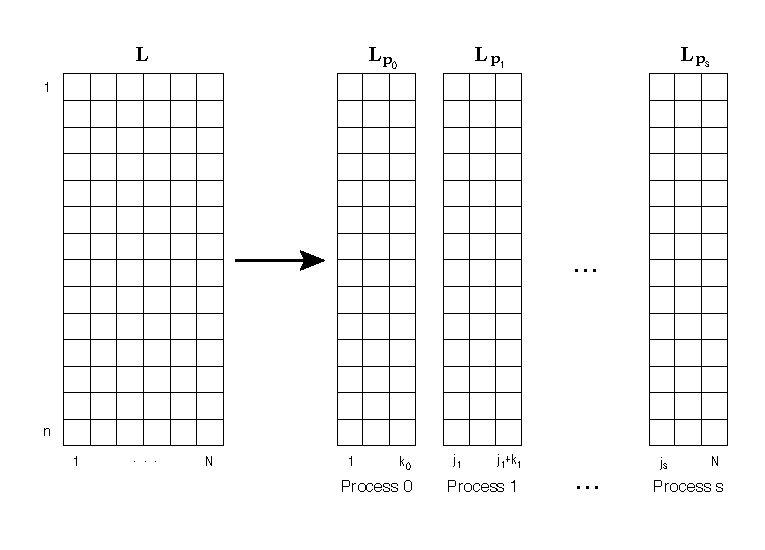
\includegraphics[width=0.8\textwidth]{figure/p91.pdf}
    \label{l_distribution}
    \caption{Distribution of the matrix $L$ into local sub-matrices $L_p$}
  \end{figure}

  \par \textcolor{red}{Parallelization of the $U$ computation}\\

  We focus in this part on the computation of the reduced covariance matrix $U$:\\
 $ U_{h+1} = U_h +  (H_{h+1}L_{h+1})^T R_{h+1}^{-1} H_{h+1}L_{h+1}$\\


  \begin{itemize}

\item The tangent observation operator is applied in parallel on each column of the local sub matrix $L_p$ (see Figure \ref{matrix_1}). The resulted matrix $HL_p$ is a sub-matrix of $HL$. The columns of $HL_p$ correspond to the same column indices as those available of matrix $HL_p$.

\begin{figure}[htpb]
        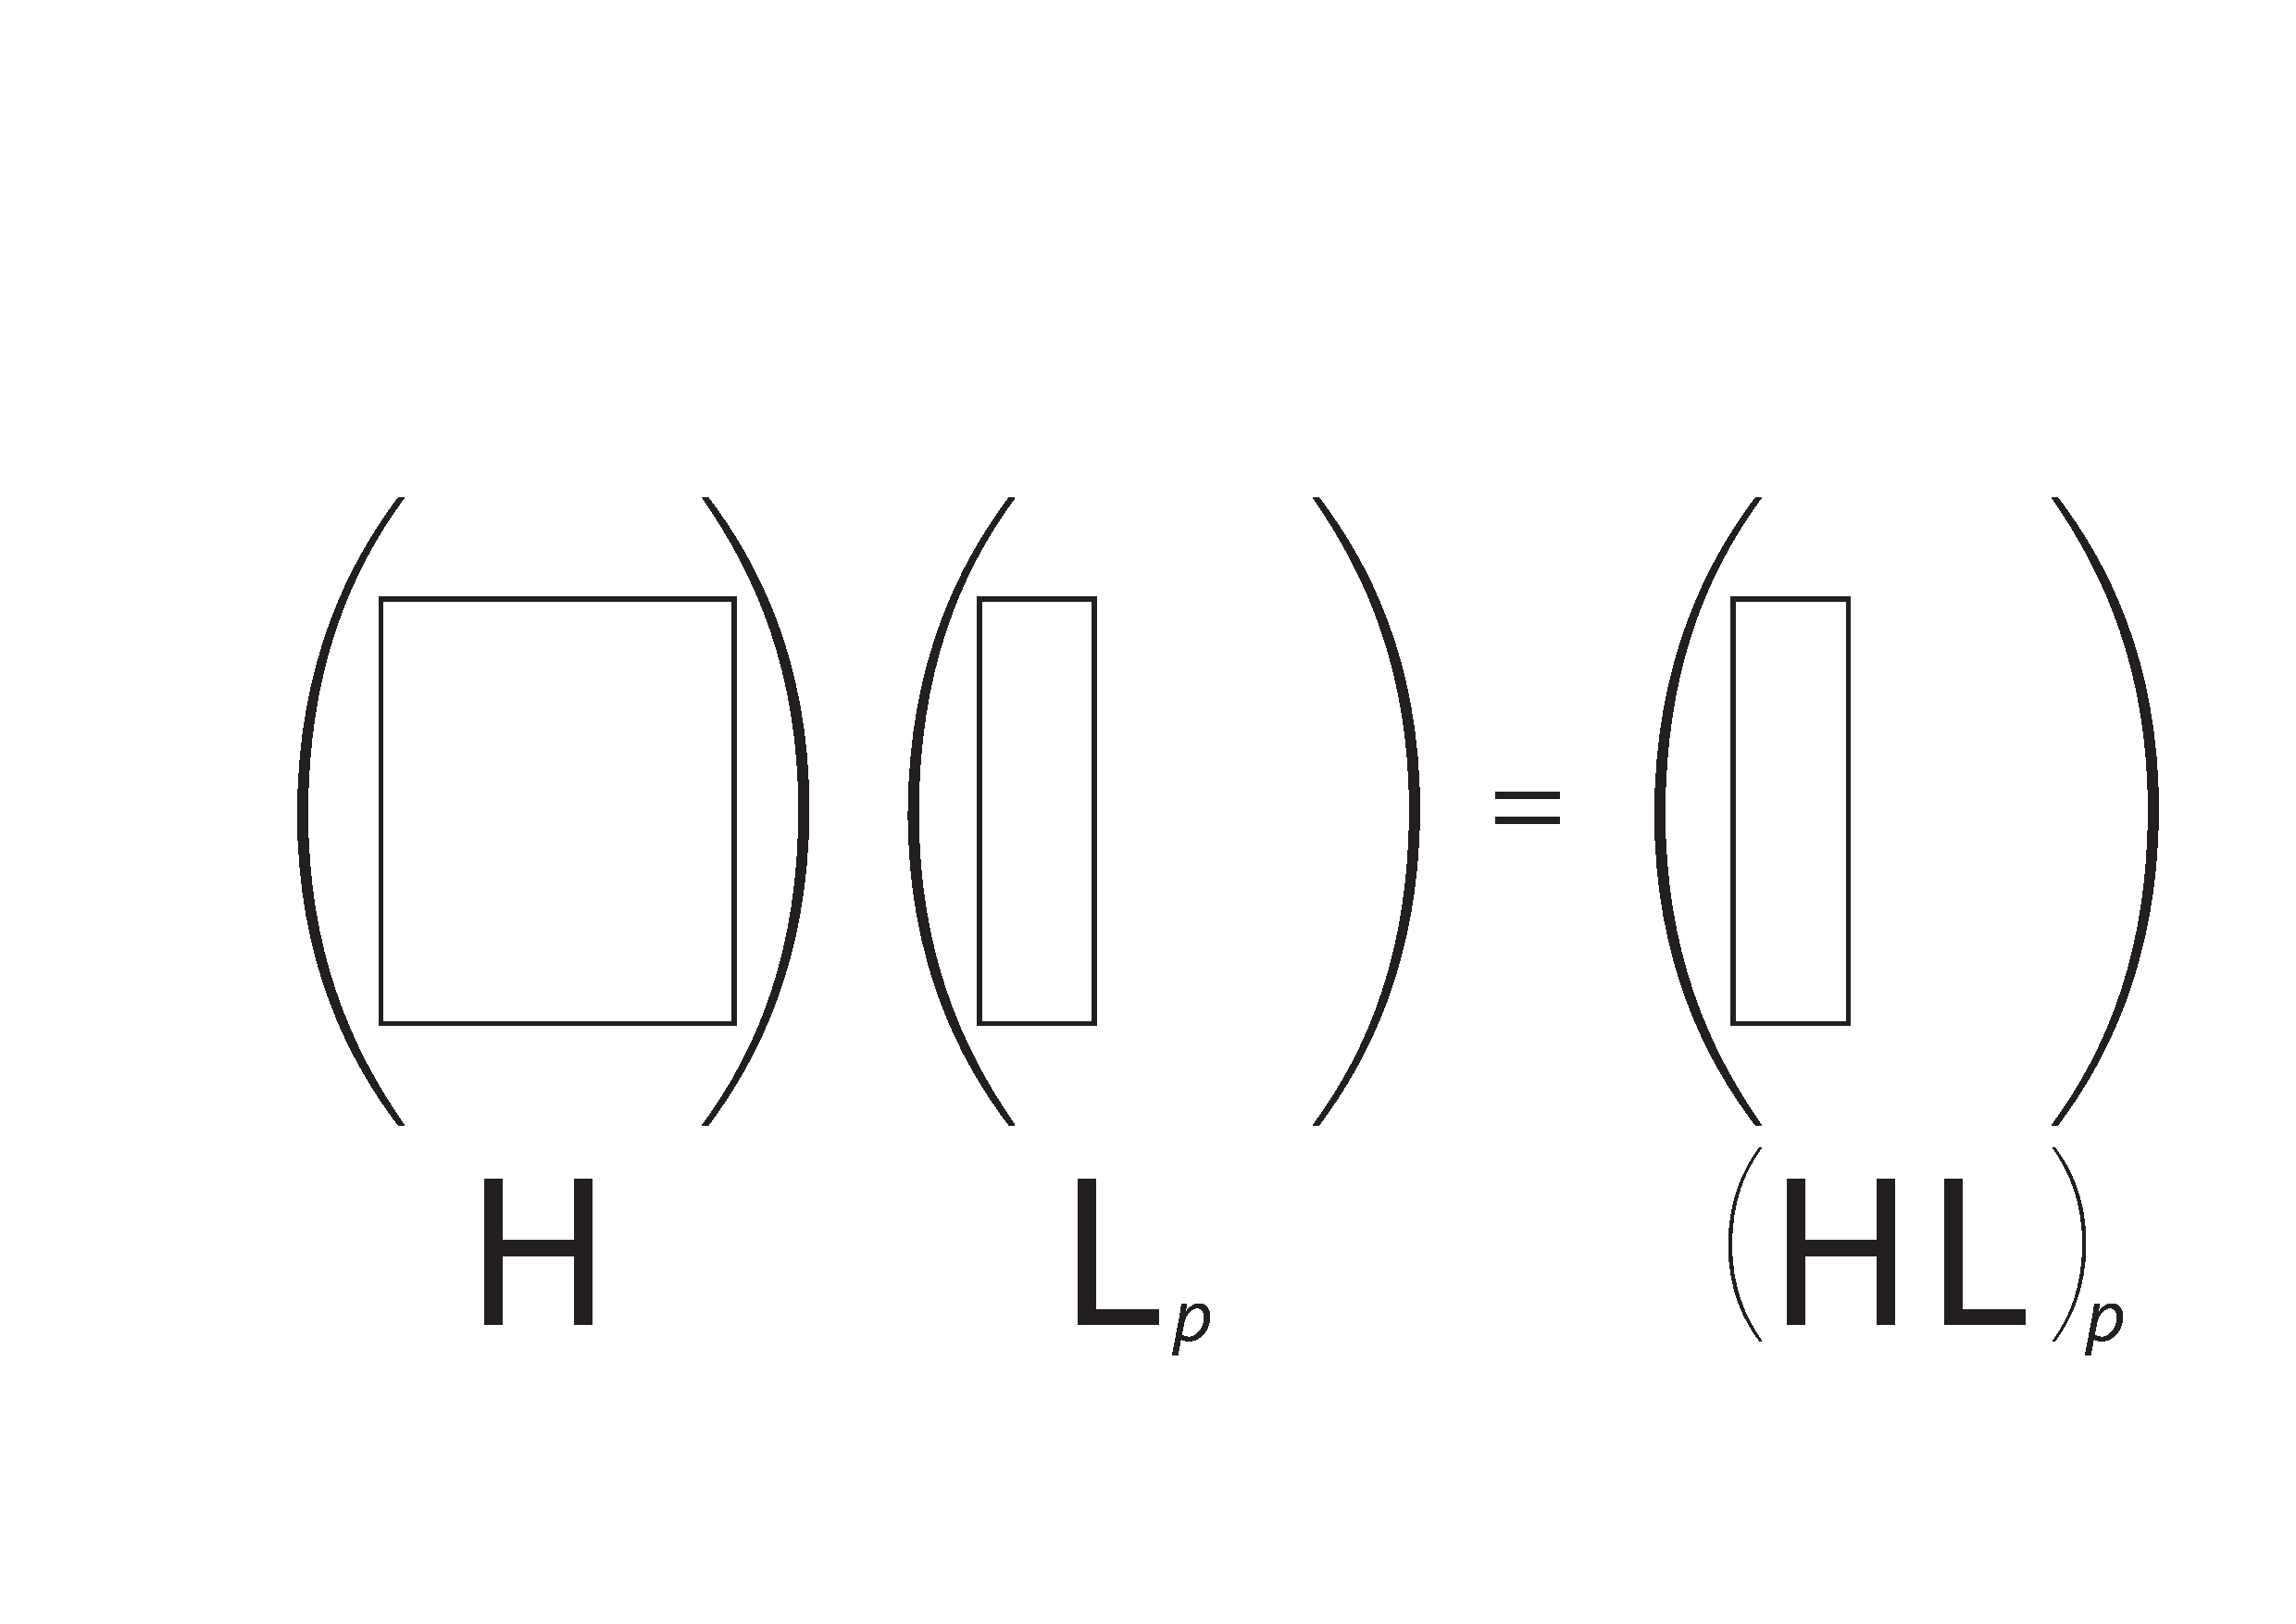
\includegraphics[width=0.6\textwidth]{figure/p92.pdf}
        \caption{Matrix-matrix product type 1}
        \label{matrix_1}
\end{figure}


\item Each process sends its local sub-matrix $HL_p$ to all others (allgather operation). Thus, each process owns the entire matrix  $HL$.\\

\item Each process computes the sub-matrix  $(R_{h+1}^{-1} H_{h+1}L_{h+1})_p$ of  $R_{h+1}^{-1} H_{h+1}L_{h+1}$ :\\
$(R_{h+1}^{-1} H_{h+1}L_{h+1})_p = R_{h+1}^{-1} (H_{h+1}L_{h+1})_p$ (see Figure \ref{matrix_1})

\item Each process computes the sub-matrix   $(U_{h+1})_p$  of  the reduced covariance matrix $U_{h+1}$:\\
 $ (U_{h+1})_p = (U_h)_p +  (H_{h+1}L_{h+1})^T (R_{h+1}^{-1} H_{h+1}L_{h+1})_p$ (see Figure \ref{matrix_1})

 \item Each process sends its local sub-matrix  $ (U_{h+1})_p$ to all others (allgather operation). Thus, each process owns the entire matrix  $U_{h+1}$.\\

\end{itemize}



\par \textcolor{red}{Parallelization of the $x^a$ computation}\\

Below is explained the update of the model state vector:\\
$ x_{h+1}^a = x_{h+1}^f + L_{h+1}U_{h+1}^{-1}(H_{h+1}L_{h+1})^T R_{h+1}^{-1} (y_{h+1}-H_{h+1}x_{h+1}^f)$\\


 \begin{itemize}
  \item Each process computes the innovation: $z = (y_{h+1}-H_{h+1}x_{h+1}^f)$.

  \item  The computation $d_p = (R_{h+1}^{-1}H_{h+1}L_{h+1})_p^Tz$  is performed in parallel by each process. Only $k_p$ rows of matrix  $(R^{-1}HL)^T$  are available locally (transpose of a matrix distributed by column). The innovation vector $z$ is fully allocated on each process. Consequently, each process is able to compute locally the $k_p$ elements of the vector $d$ whose indices correspond to those of the row of $(R^{-1}HL)^T$ available locally  (see \ref{matrix_2}).

  \item Each process sends its local sub-vector  $d_p$ to all others (allgather operation). Thus, each process owns the entire vector  $d$.\\

    \begin{figure}[htpb]
        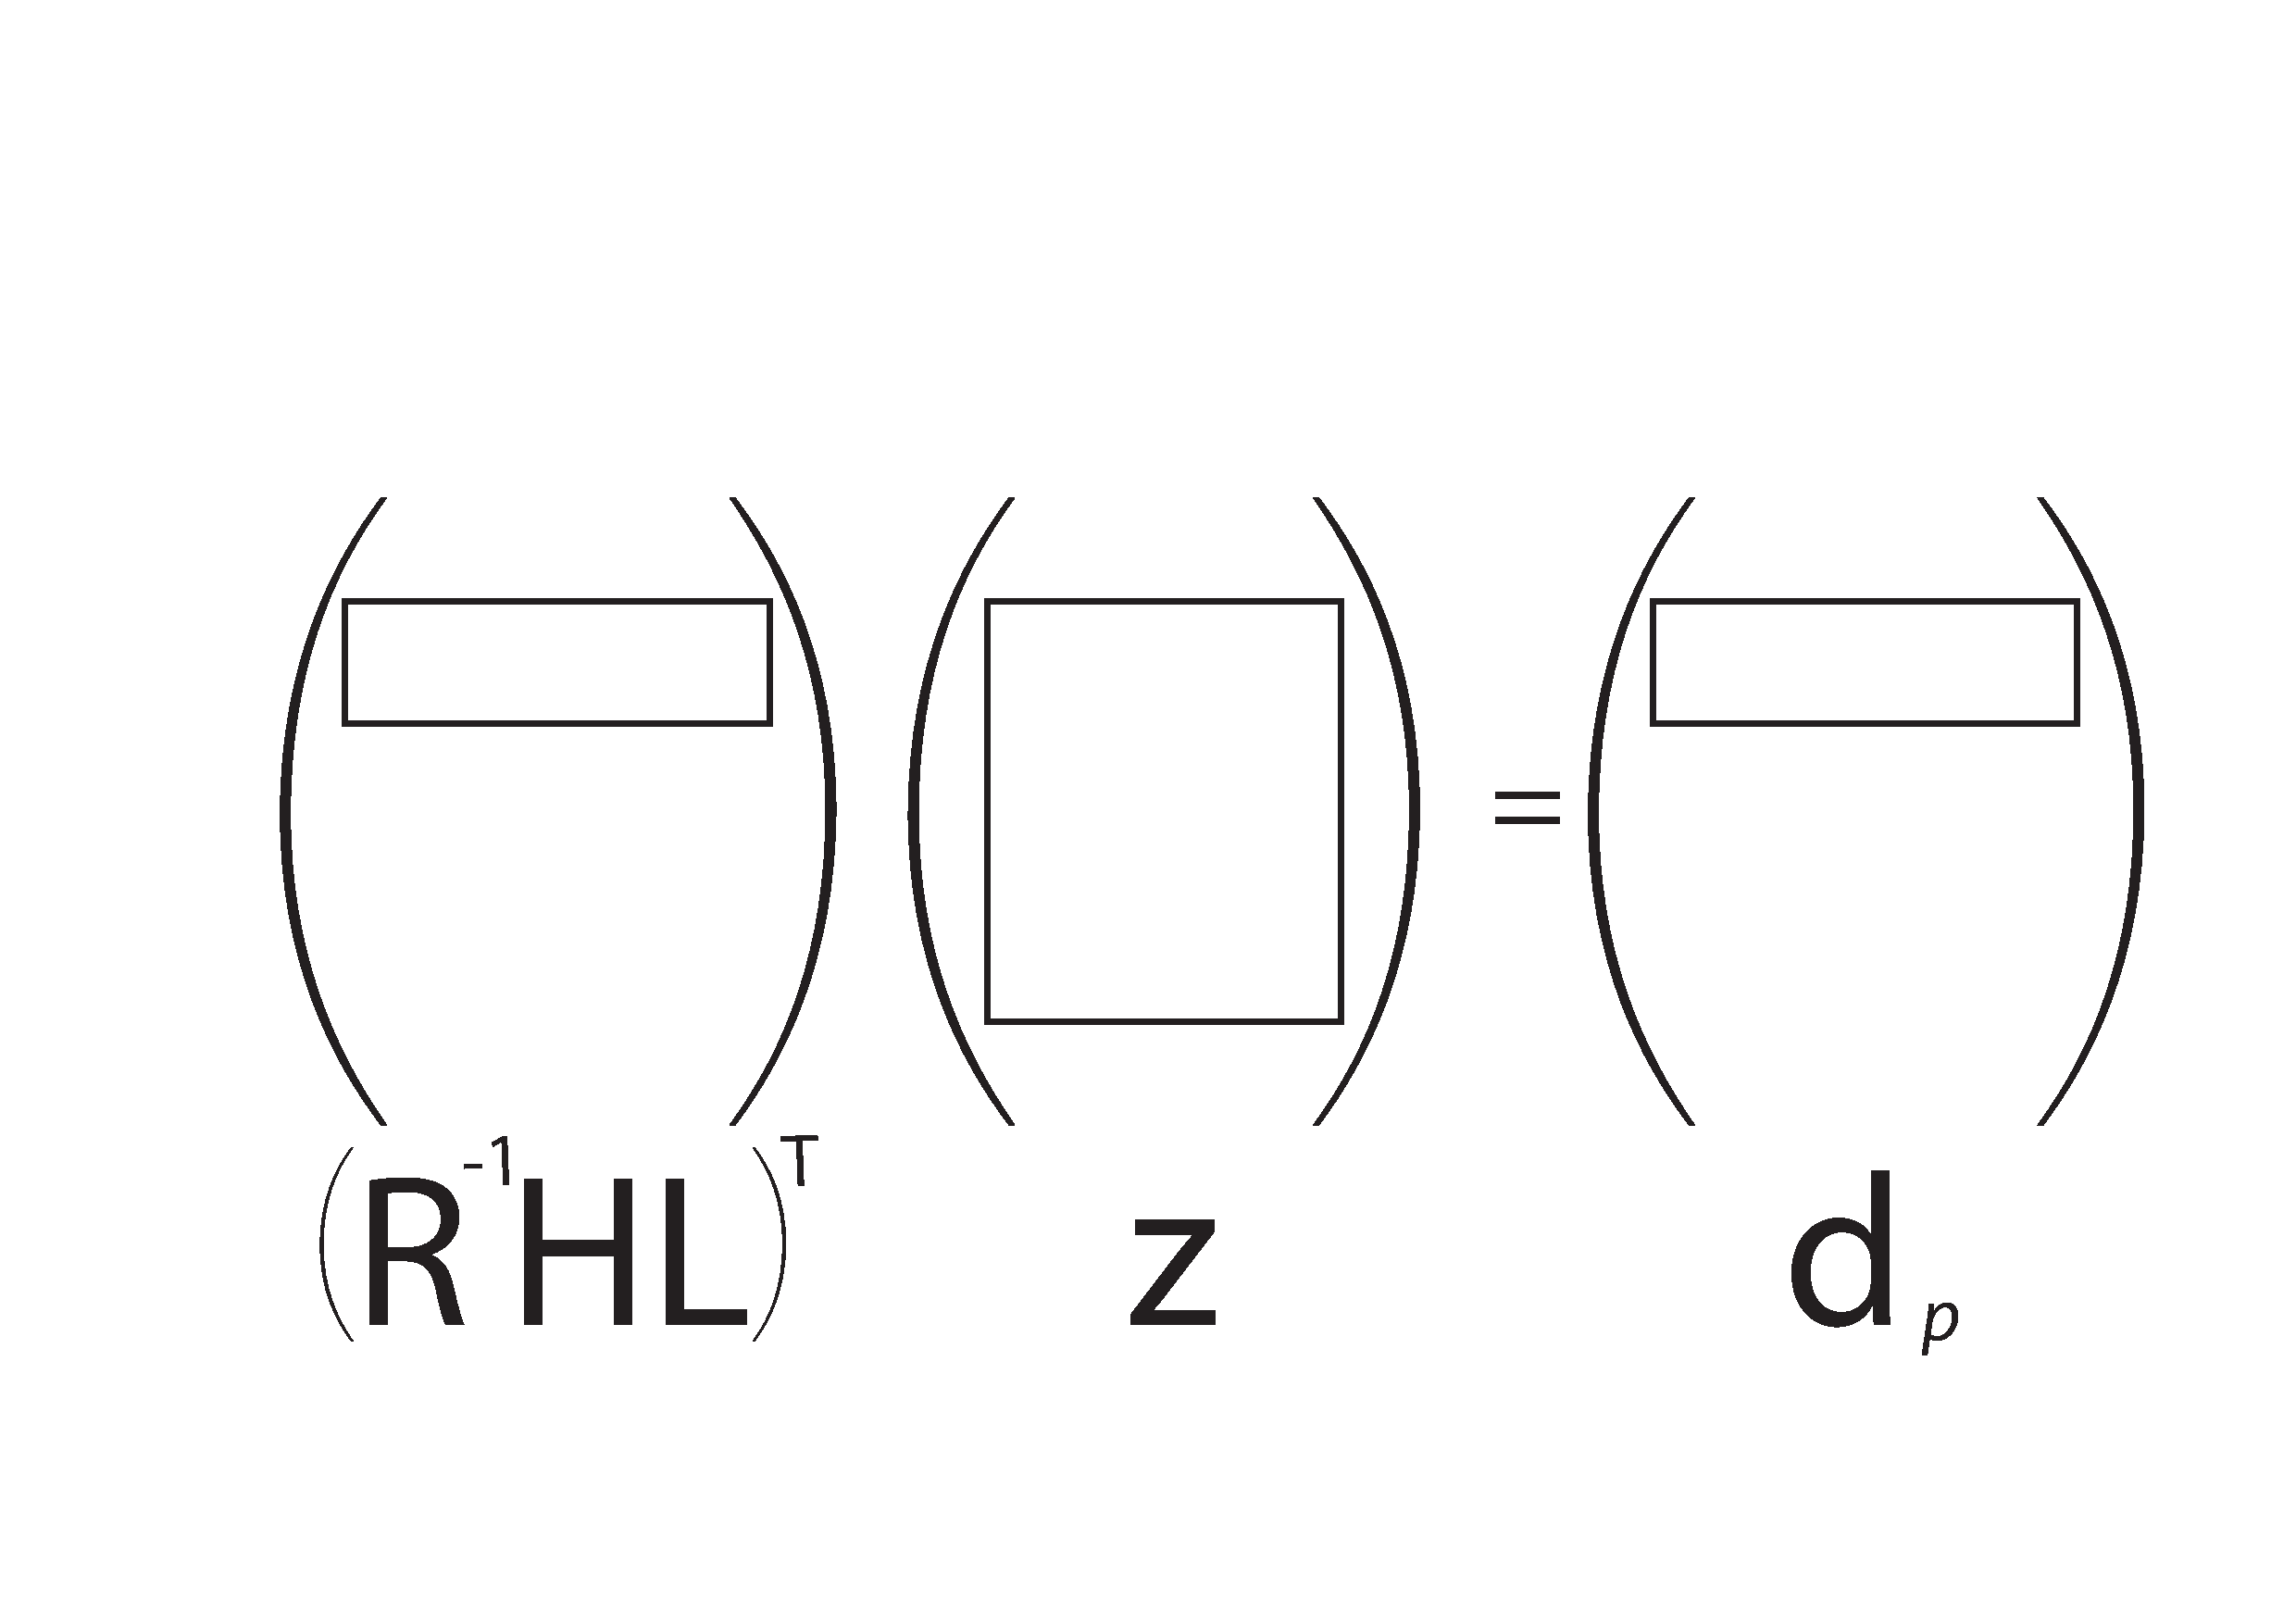
\includegraphics[width=0.6\textwidth]{figure/p93.pdf}
        \caption{Matrix-matrix product type 2}
        \label{matrix_2}
      \end{figure}

 \item The system  $U_{h+1}c = d$ is solved by each process.

  \item Each process computes computes the local contribution $\Delta x_p = (L_{h+1})_p c$ :\\
  Only $k_p$ columns of matrix $L_{h+1}$ and $k_p$ rows of vector $c$ are available locally. The product $\Delta x_p = (L_{h+1})_p c$ is a vector of the same size of $x^a$ which elements represent a partial sum of the product $L_{h+1} c$ (see Figure \ref{matrix_3}). Thus, to obtain the product  $L_{h+1} c$, the contribution of all the processes have to be summed (all reduce operation).

     \begin{figure}[htpb]
        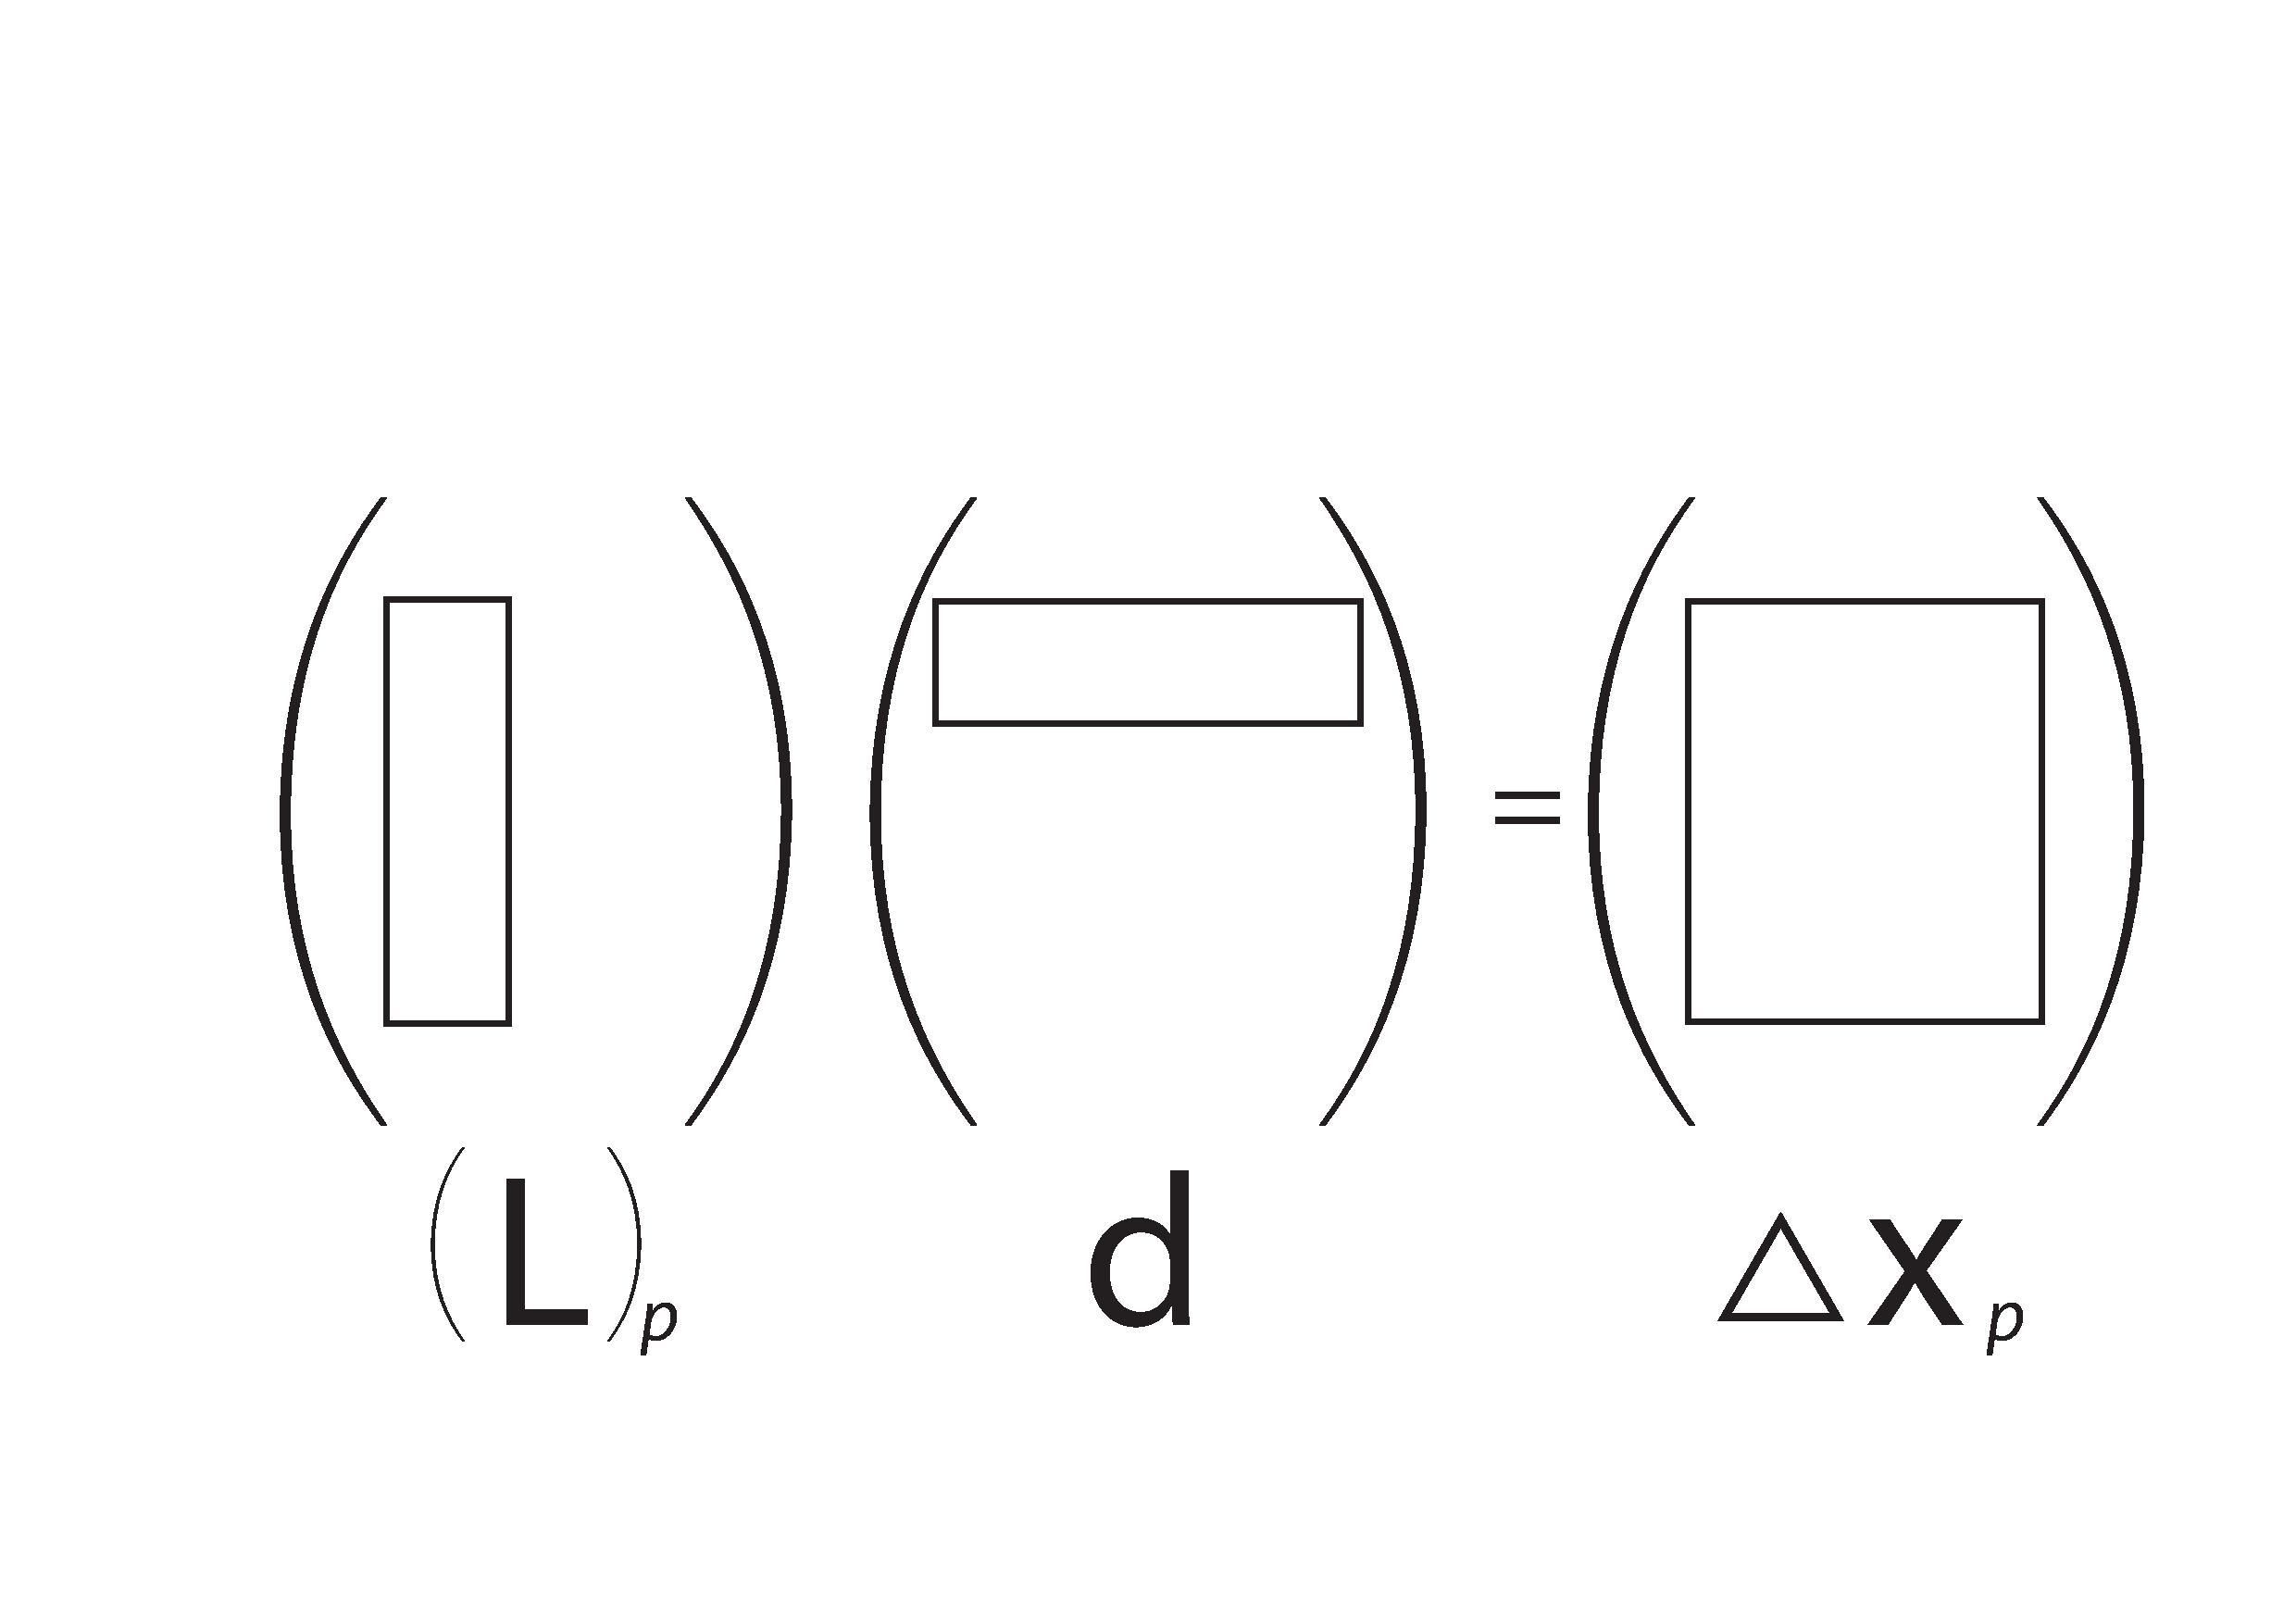
\includegraphics[width=0.6\textwidth]{figure/p94.pdf}
        \caption{Matrix-matrix product type 3}
        \label{matrix_3}
\end{figure}



  \end{itemize}


\hypertarget{par-seq-algo-roukf}{}\paragraph{Parallelization of the 'ReducedOrderUnscentedKalmanFilter'}\label{par-seq-algo-roukf}

  \par \textcolor{red}{Algorithm}\\


  \begin{DoxyEnumerate}
\item \-Sampling\-:
\begin{DoxyItemize}
\item $ C_{h} = \sqrt{U_h^{-1}} $\par

\item $ x_{h}^{(i)a} = x_h^a + L_hC_hI^{(i)} \textrm{, } \quad 1\leq i \leq p+1 $\par

\end{DoxyItemize}
\item \-Prediction\-:
\begin{DoxyItemize}
\item $ x_{h+1}^f = E_\alpha(\mathcal{M}_{h}(x_{h+1}^{(*)a})) $\par

\item $ x_{h+1}^{(i)f} = x_{h+1}^f + [\mathcal{M}_{h}(x_{h}^{*a}) - x_{h+1}^f]D_{\alpha}^{1/2} \Upsilon_p I^(i), \textrm{ resampling with SVD} $\par

\item $ L_{h+1} = [x_{h+1}^{(*)f}]D_\alpha [V^*]^T \in \mathcal{M}_{n,p} $\par

\item $ P_{h+1}^f = L_{h+1} (P_{\alpha}^V)^{-1} L_{h+1}^T $
\end{DoxyItemize}
\item \-Update\-:
\begin{DoxyItemize}
\item $ [\tilde{y}] = [\mathcal{H}_{h+1}(x_{h+1}^{(*)f}) - E_\alpha(\mathcal{H}_{h+1}(x_{h+1}^{(*)f})) ]$\par

\item $ D_m = [\tilde{y}]^T R_{h+1}^{-1}[\tilde{y}] \in \mathcal{M}_r $\par

\item $ U_{h+1} = P_{\alpha}^V + [V^*] D_\alpha \bigl(1 + D_m(D_\alpha - D_V)\bigr)^{-1} D_m D_\alpha [V^*]^T \in \mathcal{M}_{p} $\par

\item $ \{HL\}_{h+1} = [\tilde{y}]( 1 + D_\alpha D_m)^{-1}\Bigl(1 + D_V \bigl( 1+D_m (D_\alpha-D_V) \bigr)^{-1} D_m \Bigr) D_\alpha[V^*]^T $\par

\item $ x_{h+1}^a = x_{h+1}^f + L_{h+1}U_{h+1}^{-1}\{HL\}_{h+1}^T R_{h+1}^{-1} (y_{h+1}-E_\alpha(y_{h+1}^{(*)}))$\par

\item $ P_{h+1}^a = L_{h+1} U_{h+1}^{-1} L_{h+1}^T$
\end{DoxyItemize}
\end{DoxyEnumerate}\-With\-: \par
 $x_h^f$ forecast state vector; \par
 $x_h^a$ analysis state vector; \par
 $y_h$ observation vector; \par
 $\mathcal{H}_h$ observation operator that maps the state space to the observation space; \par
 $H_h$ observation operator linearized at $x^f_h$; \par
 $P^f_h$ error covariance matrix of $x_h^f$; \par
 $P^a_h$ error covariance matrix of $x_h^a$; \par
 $R_h$ observational error covariance matrix; \par
 $\mathcal{M}_h$ model.



 \begin{itemize}
  \item  The particles  $x_{h}^{(i)a}$ are distibuted over the processes.
  \item Each process executes the sequential ROUKF algorithm with its local particles.
  \item The matrices $x_{h+1}$, $L_{h+1}$, $(HL)_{h+1}$ et $U_{h+1}$ are updated with the different parallel matrix-matrix products presented in Section \ref{par-seq-algo-roekf}.
  \end{itemize}


\hypertarget{par-seq-example}{}\subsection{Example Programs}\label{par-seq-example}


The examples are located in the {\ttfamily example/clamped\_bar} directory.\footnote{To have a summary of \emph{Verdandi} contents see Section \ref{overview}.}


\hypertarget{par-seq-example-compilation}{}\paragraph{Compilation}\label{par-seq-example-compilation}

First of all, the preprocessor variable $ VERDANDI\_WITH\_MPI $ has to be defined in files  \textbf{reduced\_order\_extended\_kalman\_filter.cpp} and \textbf{reduced\_order\_unscented\_kalman\_filter.cpp}:

\begin{frame_cpp}
#define VERDANDI_DEBUG_LEVEL_4
#define SELDON_WITH_BLAS
#define SELDON_WITH_LAPACK

#define VERDANDI_WITH_ABORT
#define VERDANDI_DENSE

#define VERDANDI_WITH_MPI

#if defined(VERDANDI_WITH_MPI)
#include <mpi.h>
#endif


#include "Verdandi.hxx"
#include "seldon/SeldonSolver.hxx"

#include "model/ClampedBar.cxx"
#include "observation_manager/LinearObservationManager.cxx"
#include "method/ReducedOrderUnscentedKalmanFilter.cxx"


int main(int argc, char** argv)
{

    VERDANDI_TRY;

    ...
}
\end{frame_cpp}

Then, compile the program \textbf{generate\_observation.cpp}:


\begin{frame_bash}
$ scons generate_observation
\end{frame_bash}

Finally, compile the programs \textbf{reduced\_order\_extended\_kalman\_filter.cpp} and \textbf{reduced\_order\_unscented\_kalman\_filter.cpp}  with the option 'mpi=yes':
\begin{frame_bash}
$ scons reduced_order_extended_kalman_filter mpi=yes
$ scons reduced_order_unscented_kalman_filter mpi=yes
\end{frame_bash}



\hypertarget{par-seq-example-observation}{}\paragraph{Observation}\label{par-seq-example-observation}

\-Since no observations are given yet, we have to generate some. \-Execute the following command\-:
\begin{frame_bash}
host<~/> ./generate_observation configuration/truth.lua
\end{frame_bash}
  to run the model with the initial conditions described in {\ttfamily truth.\-lua}, without data assimilation. \-This should generate a result file ({\ttfamily truth-\/state\-\_\-forecast.\-bin}) in the directory {\ttfamily example/clamped\-\_\-bar/result/}. \-This file store the state (displacement, velocity, $ \theta_{f} $) trajectory.

\-The generated state (displacement, velocity, $ \theta_{f} $) will serve as observations for the assimilation.



\hypertarget{par-seq-example-dam}{}\paragraph{Data Assimilation with ROEKF and ROUKF}\label{par-seq-example-dam}


\-To use the \hyperlink{reduced_order_extended_kalman_filter}{\-Reduced \-Order \-Extended \-Kalman \-Filter} and the \hyperlink{reduced_order_unscented_kalman_filter}{\-Reduced \-Order \-Unscented \-Kalman \-Filter} methods, execute the following commands.
\begin{frame_bash}
$ mpirun -n 2 reduced_order_extended_kalman_filter configuration/assimilation.lua
$ mpirun -n 2 reduced_order_unscented_kalman_filter configuration/assimilation.lua
\end{frame_bash}
  \-This runs the model with the initial conditions described in {\ttfamily example/clamped\-\_\-bar/configuration/assimilation.\-lua}. \-The simulation begins with erroneous values for the parameter $ \theta_f $. \-This should generate the same results as for the sequential simulation.\\


  \textbf{Warning:}  The number of processes should be less than or equal to the size of the reduced model state vector.



\hypertarget{par-seq-performance}{}\subsection{Performance}\label{par-seq-performance}

The figures \ref{titre2} and \ref{titre3} introduce the resulting performance of the ROEKF and ROUKF algorithms applied to the sequential model ClampedBar. These simulations were performed on 2 x 3 GHz Quad-Core Intel Xeon with a 16 GB of memory in which the processes used during simulation were placed at arbitrary cores relative to the process constructing the network.

\begin{figure}
    \caption{\label{titre2} Speed up of the parallel ROEKF algorithm applied to the sequential model ClampedBar with $N_{state} = 10^4$, $N_{observation} = 10^2$ and $N_{sigma\_point} = 16$.}

 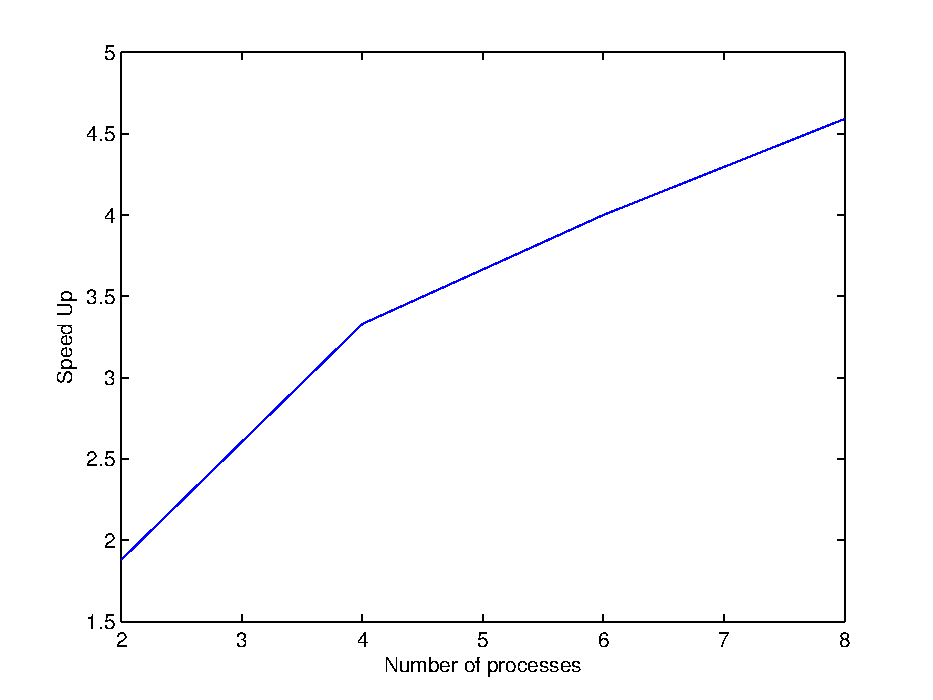
\includegraphics[width=0.8\textwidth]{figure/speed_up_roekf.pdf}

   \end{figure}



 \begin{figure}
  \caption{\label{titre3} Speed up of the parallel ROUKF algorithm applied to the sequential model ClampedBar with $N_{state} = 10^4$, $N_{observation} = 10^2$ and $N_{sigma\_point} = 16$.}

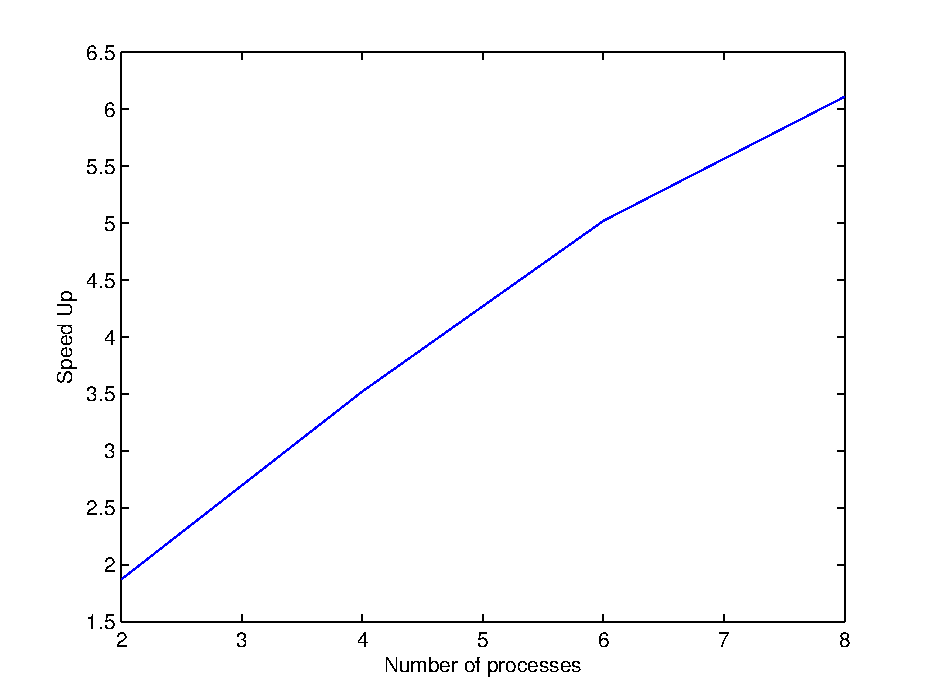
\includegraphics[width=0.8\textwidth]{figure/speed_up_roukf.pdf}

\end{figure}


\newpage


\hypertarget{seq-par}{}\section{Sequential Method applied to Parallel Model}\label{seq-par}

Verdandi intends to provide the ability to apply its data assimilation methods to models whose state vector is distributed on several processes. In the case of large scale state vector, neither the model nor the data assimilation method can afford to allocate a variable of this size. Consequently, several data assimilation variables
could be distributed, for instance the sensitivity matrix and the variance. The number of components to be stored locally has to be compatible with the distributed model state vector for parallel matrix-vector operations.

The management of the types in Verdandi, detailed in Section \ref{seq-par-type}, enabled to implement this capability easily. The chosen solution was to create an interface between Seldon, the linear algebra library used in Verdandi, and PETSc a framework for parallel computing. This choice do not confine the type of the model state vector only to PETSc distributed structures since any MPI distributed structures can be encapsulated or copied in a PETSc object.


\hypertarget{seq-par-type}{}\subsection{Types Management in Verdandi}\label{seq-par-type}


The implementation of the Verdandi algorithms relies on the linear algebra library Seldon. This library provides different matrix and vector structures, and many functions for computations (linear algebra). It provides matrices for two main categories: dense matrices and sparse matrices. Among dense matrices, there are specific structures for rectangular matrices, symmetric matrices, hermitian matrices and triangular matrices. Each type includes several formats: rectangular dense matrices may be stored by rows or by columns; symmetric dense matrices may be stored as rectangular matrices or only upper part of the matrix is stored. Many different types
for sparse matrix are also available. All  of these matrix classes share the same interface. Linear algebra computation functions are template functions and many BLAS operations bringing into play different matrix types are implemented.


Example program which computes the product of a dense matrix by a sparse matrix:


\begin{frame_cpp}
// Dense  matrix.
Matrix<double, General, RowMajor> A(3, 3), C(3, 3);
A.Fill();
C.Fill();
// Sparse matrix.
Matrix<double, General, ArrayRowSparse> B(3, 3);
B(0, 0) = 2.0;
B(1, 0) = 1.0;
// Computes matrix-matrix product alpha*A*B + beta*C -> C.
// This function is overloaded for all types of matrices.
MltAdd(1.0, A, B, 2.0, C);
\end{frame_cpp}


In Verdandi, the model and the observation manager can provide their vector and matrix types to the data assimilation method thanks to the C++ 'typedef' mechanism. For instance :


\begin{frame_cpp}
class Model
{
    public:
        //! Type of the state error variance.
        typedef Matrix<double, General, RowSparse> state_error_variance;
        /*! \brief Type of the reduced matrix \f$U\f$ in the \f$LUL^T\f$
        decomposition of the state error variance. */
        typedef Matrix<double, General, RowMajor> state_error_variance_reduced;
        //! Type of the state vector.
        typedef Vector<double> state;
	...
}
\end{frame_cpp}


\begin{frame_cpp}
class ObservationManager
{
    public:
        //! Type of the tangent linear operator.
        typedef Matrix<double, General, RowSparse> tangent_linear_operator;
        //! Type of the observation vector.
        typedef Vector<double> observation;
	...
}
\end{frame_cpp}


Thus, the data assimilation method is able to get back the type of the object to instantiate. For instance, to fetch the type of the model state vector:

\begin{frame_cpp}
template <class Model, class ObservationManager>
class DataAssimilationMethod
{
...
        //! Type of the model state vector.
        typedef typename Model::state model_state;
...
}
\end{frame_cpp}



\hypertarget{seq-par-ds}{}\subsection{Distributed Structure in Seldon}\label{seq-par-ds}


To ensure the compatibility of the Verdandi data assimilation methods with distributed models,  it was sufficient to:

\begin{itemize}

\item add vector and matrix distributed structures to Seldon.

\item implement the linear algebra computation functions for these new types, required by the concerned data assimilation methods.

\end{itemize}

\hypertarget{seq-par-ds-vector}{}\paragraph{Distributed Vector}\label{seq-par-ds-vector}


The class Seldon$::$Vector$<$double, PETScPar$>$  encapsulate a distributed PETSc vector of type \textbf{VecMPI} . This class implement the same interface as a classic Seldon vector. The whole set of BLAS1 operations have been implemented for this type.

The source files of the class Seldon$::$Vector$<$double, PETScPar$>$  are located in the seldon/vector/ directory. Several methods are specific of  Seldon$::$Vector$<$double, PETScPar$>$ class:

\begin{frame_cpp}
template <class T, class Allocator>
class Vector<T, PETScPar, Allocator>: public PETScVector<T, Allocator>
{
	...

    // Returns a reference on the inner petsc vector.
    Vec& GetPetscVector();

    // Returns a const reference on the inner petsc vector.
    const Vec& GetPetscVector() const;

    // Sets the MPI communicator.
    void SetCommunicator(MPI_Comm mpi_communicator);

    // Inserts or adds values into certain locations of a vector.
    // \warning These values may be cached, so 'Flush' must be called after
    // all calls to SetBuffer() have been completed.
    void SetBuffer(int i, T value, InsertMode insert_mode = INSERT_VALUES);

    // Assembles the PETSc vector.
    void Flush();

    // Returns the range of indices owned by this processor.
    // The vectors are laid out with the first \f$n_1\f$ elements on the first
    // processor, next \f$n_2\f$ elements on the second, etc. If the current
    // processor is \f$k\f$, this method returns \f$n_k\f$ in \a i and
    // \f$n_{k+1}\f$ in \a j. If \a i is set to PETSC_NULL on entry, it is not
    // modified by this function. Same is true for \a j.
    void GetProcessorRange(int& i, int& j) const;

    ...
}
\end{frame_cpp}


\par These specific methods may be necessary during the construction of a distributed vector. These methods are never called by data assimilation methods which delegate the distributed variable initializations to models and observation managers.


\textbf{Distributed PETSc vector example program}


\begin{frame_cpp}

    Vec x, y;

    int N = 10;

    ierr = VecCreateMPI(PETSC_COMM_WOLRD, N, &x); CHKERRQ(ierr);
    ierr = VecCreateMPI(PETSC_COMM_WOLRD, N, &y); CHKERRQ(ierr);
    ierr = VecSet(x, 3.0); CHKERRQ(ierr);
    ierr = VecSet(y, 1.0); CHKERRQ(ierr);

    ierr = VecAssemblyBegin(x); CHKERRQ(ierr);
    ierr = VecAssemblyEnd(x); CHKERRQ(ierr);
    ierr = VecAssemblyBegin(y); CHKERRQ(ierr);
    ierr = VecAssemblyEnd(y); CHKERRQ(ierr);

    ierr = VecAXPY(y, -1.0, x); CHKERRQ(ierr);

    ierr = VecDestroy(&x); CHKERRQ(ierr);
    ierr = VecDestroy(&y); CHKERRQ(ierr);


\end{frame_cpp}


\textbf{The same example using the Vector$<$double, PETScPar$>$ class}

\begin{frame_cpp}

    Vector<double, PETScPar> x, y;
    x.Reallocate(10);
    y.Reallocate(10);
    x.Fill(3.);
    y.Fill(1.);

    Add(-1., x, y);

\end{frame_cpp}


\hypertarget{seq-par-ds-dmatrix}{}\paragraph{Distributed Dense Matrix}\label{seq-par-ds-dmatrix}


The class Seldon$::$Matrix$<$T, Prop, PETScMPIDense, Allocator$>$  encapsulate a  dense distributed PETSc matrix of type \textbf{MATMPIDENSE} . This class implement the same interface as a classic Seldon matrix.

The source files of the class Seldon$::$Matrix$<$T, Prop, PETScMPIDense, Allocator$>$   are located in the seldon/matrix/ directory. Several methods are specific of  Seldon$::$Matrix$<$T, Prop, PETScMPIDense, Allocator$>$  class:


\begin{frame_cpp}
template <class T, class Prop, class Allocator>
class Matrix<T, Prop, PETScMPIDense, Allocator>:
public PetscMatrix<T, Prop, RowMajor, Allocator>
{
	...

    // Returns a reference on the inner petsc matrix.
    Mat& GetPetscMatrix();
    // Returns a const reference on the inner petsc matrix.
    const Mat& GetPetscMatrix() const;


    // Sets the MPI communicator.
    void SetCommunicator(MPI_Comm mpi_communicator);
    // Returns the MPI communicator of the current PETSc matrix.
    MPI_Comm GetCommunicator() const;

    // Inserts or adds values into certain locations of a matrix.
    // \warning These values may be cached, so 'Flush' must be called after all
    // calls to SetBuffer() have been completed.
    void SetBuffer(int, int, T, InsertMode);

    // Assembles the PETSc matrix.
    void Flush() const;

    // Returns the range of row indices owned by this processor.
    // The matrix is laid out with the first \f$n_1\f$ rows on the first
    // processor, next \f$n_2\f$ rows on the second, etc. If the current
    // processor is \f$k\f$, this method returns \f$n_k\f$ in \a i and
    // \f$n_{k+1}\f$ in \a j. If \a i is set to PETSC_NULL on entry, it is not
    // modified by this function. Same is true for \a j.
    void GetProcessorRowRange(int& i, int& j) const;

    ...
}
\end{frame_cpp}


\par These specific methods may be necessary during the construction of a distributed matrix. These methods are never called by data assimilation methods which delegate the distributed variable initializations to models and observation managers.

\hypertarget{seq-par-ds-smatrix}{}\paragraph{Distributed Sparse Matrix}\label{seq-par-ds-smatrix}

The class Seldon$::$Matrix$<$T, Prop, PETScMPIAIJ, Allocator$>$  encapsulate a sparse distributed PETSc matrix of type \textbf{MATMPIAIJ} . This class has the same interface as the  Seldon$::$Matrix$<$T, Prop, PETScMPIDense, Allocator$>$ class  introduced previously.

The source files of the class Seldon$::$Matrix$<$T, Prop, PETScMPIAIJ, Allocator$>$   are located in the seldon/matrix/ directory



\hypertarget{seq-par-dm}{}\subsection{'PETScClampedBar' Distributed Model}\label{seq-par-dm}


Verdandi provides an implementation of the 'ClampedBar' model based on the distributed structures available in Seldon. The source files of the distributed 'PetscClampedBar' model are located in the verdandi/model/ directory.



\hypertarget{seq-par-dm-m}{}\paragraph{The 'PETScClampedBar' Model}\label{seq-par-dm-m}


The clamped bar model describes the vibration of a bar clamped at one end. The bar is discretized with $Nx$ finite elements of the same length. With the hypothesis of "small displacements", it follows the linear system:

\begin{center} $ M \ddot Y + C \dot Y + K Y = F_{\theta_f}$ \par
 \end{center}

 where $M$  is the mass matrix, $K$  is the stiffness matrix,  $C$  is the damp matrix and  $F(\theta_f) = \sin(\frac{\pi t}{t_f}) M_{\theta_f} (1 ... 1)^T$  is the effort vector.


 The clamped bar model is solved numerically using a Newmark scheme (middle point) for integration in time:

 $ \ddot Y_{h + \frac{1}{2}} = \frac{\ddot Y_{h+1} + \ddot Y_{h} }2 = \frac{\dot Y_{h+1} - \dot Y_{h} } {\Delta t} $ \par
$ \dot Y_{h + \frac{1}{2}} = \frac{\dot Y_{h+1} + \dot Y_{h} }2 = \frac{Y_{h+1} - Y_{h} } {\Delta t} $\\


Algorithmically, it follows:

$ \dot Y_{h + 1} = \frac{2}{\Delta t}(Y_{h+1} - Y_{h}) - \dot Y_{h} $ \par
$Newmark_1 = \frac{1}2K + \frac{1}{\Delta t}C + \frac{2}{\Delta t^2}M$ \par
$Newmark_0 = -\frac{1}2 K + \frac{1}{\Delta t}C + \frac{2}{\Delta t^2}M$ \par
$Newmark_1Y_{h+1} = Newmark_0Y_{h} + \frac{2}{\Delta t}M\dot Y_{h} + F_{h + \frac{1}{2}}(\theta_f)$\\

The matrices  $M$, $Newmark_0$ and $Newmark_1$ are sparse distributed matrices of type Matrix$<$T, Prop, PETScMPIAIJ, Allocator$>$. The effort vector $F$ is a distributed vector of type  Vector$<$double, PETScPar$>$:


\begin{frame_cpp}
template <class T>
class PetscClampedBar: public VerdandiBase
{
    public:

    ...

    //! Mass matrix.
    Matrix<T, General, PETScMPIAIJ> mass_;
    //! Newmark matrix 0.
    Matrix<T, General, PETScMPIAIJ> newmark_0_;
    //! Newmark matrix 1.
    Matrix<T, General, PETScMPIAIJ> newmark_1_;

    //! Force.
    Vector<T, PETScPar> rhs_;

    ...

}
\end{frame_cpp}


\hypertarget{seq-par-dm-sv}{}\paragraph{Management of the Model State Vector}\label{seq-par-dm-sv}

The model state vector contains the displacement vector $Y$, the velocity vector $\dot Y$ and the parameter vector $\theta_f$. The Table \ref{titre4} gives the distribution of the state vector over processes.


\begin{table}
    \caption{\label{titre4} Distribution of the 'PetscClampedBar' state vector over processes.}

   \vspace{1.5cm}

    \begin{tabular}{|c|c|c|c|c|}
      \hline
       & \multicolumn{4}{c|}{Processeurs}\\
      \hline
       & $0$ & $1$ & ... & $N_{process} - 1$\\
      \hline
      $Y$ & $Y^0 =  (Y_0... Y_{\frac{N_x}{N_{process}} -1})$ &   $Y^1 = (Y_{\frac{N_x}{N_{process} }} ... Y_{2.\frac{N_x}{N_{process}} - 1 })$ & ... &  $(Y_{\frac{(N_{process} - 1).N_x}{N_{process} }} ... Y_{N_x - 1 })$\\
      \hline
      $\dot Y$ & $\dot Y^0 =  (\dot Y_0 ... \dot Y_{\frac{N_x}{N_{process}} -1})$ & $\dot Y^1 = (\dot Y_{\frac{N_x}{N_{process} }} ... \dot Y_{2.\frac{N_x}{N_{process}} - 1 })$ & ... & $(\dot Y_{\frac{(N_{process} - 1).N_x}{N_{process} }} ... \dot Y_{N_x - 1 })$ \\
      \hline
     $\theta_f$ &  & & &  $\theta_f$ \\
     \hline
    \end{tabular}
  \end{table}


The displacement vector $Y$ and the velocity vector $\dot Y$ are distributed vectors. The parameter vector $\theta_f$ is a sequential vector stored on the process of rank $Nprocess - 1$. When $\theta_f$ is updated, this process is responsible for sending the updated vector $\theta_f$ to all other.


\begin{frame_cpp}
template <class T>
class PetscClampedBar: public VerdandiBase
{
    public:

        ...

        //! Type of the model state vector.
        typedef Vector<T, PETScPar> state;
        //! Type of the model parameter vector.
        typedef Vector<T> parameter;


        //! Displacement.
        state displacement_0_;
        //! Velocity.
        state velocity_0_;
        //! Force parameter.
        parameter theta_force_;

         //! Local size of state vector.
        int Nstate_local_;
        //! Model state.
        state state_;

        ...

}
  \end{frame_cpp}



\par \textcolor{red}{GetState}\\


The model state vector is passed to the data assimilation method by local copy:


$X^i = (Y^i, \dot Y^i), 0 \le i \le N_{process} - 2 $ \par
$X^{N_{process} - 1} = (Y^{N_{process} - 1}, \dot Y^{N_{process} - 1}, \theta_f)$


 \begin{frame_cpp}
template <class T>
typename PetscClampedBar<T>::state& PetscClampedBar<T>
::GetState()
{
    int disp_start, disp_end;
    displacement_0_.GetProcessorRange(disp_start, disp_end);
    int state_start, state_end;
    state_.GetProcessorRange(state_start, state_end);
    for (int i = disp_start; i < disp_end; i++)
    {
        state_.SetBuffer(state_start++, displacement_0_(i));
        state_.SetBuffer(state_start++, velocity_0_(i));
    }
    if (rank_ == Nprocess_ - 1)
        for (int j = 0; j < parameter_.GetVector(reduced_[i]).GetSize(); j++)
            state_.SetBuffer(state_start++, theta_force_(j));
    state_.Flush();
    return state_;
}
  \end{frame_cpp}



\par \textcolor{red}{StateUpdated}\\


When the model state vector is updated, it is necessary to update the vectors $Y$ and $\dot Y$. The process $N_{process} - 1$ must broadcast the updated vector $\theta_f$ to all other processes.

\begin{frame_cpp}
template <class T>
void PetscClampedBar<T>
::StateUpdated()
{
    int disp_start, disp_end;
    displacement_0_.GetProcessorRange(disp_start, disp_end);
    int state_start, state_end;
    state_.GetProcessorRange(state_start, state_end)
    for (int i = disp_start; i < disp_end; i++)
    {
        displacement_0_.SetBuffer(i, state_(state_start++));
        velocity_0_.SetBuffer(i, state_(state_start++));
    }
    if (rank_ == Nprocess_ - 1)
        for (int j = 0; j < Ntheta_force_; j++)
            theta_force_(j) = state_(state_start++);
    displacement_0_.Flush();
    velocity_0_.Flush();
    MPI_Bcast(theta_force_.GetData(), Ntheta_force_, MPI_DOUBLE, Nprocess_ - 1, mpi_communicator_);
}
\end{frame_cpp}



\hypertarget{seq-par-dm-cm}{}\paragraph{Covariance Matrix}\label{seq-par-dm-cm}

The 'PetscClampedBarModel' provides a decomposition of the state error covariance matrix ($P$) as a product $LUL^T$.

The matrix $U$ is a matrix of small size, it is implemented as a sequential dense matrix.

The matrix $L$ is a matrix of $\mathcal{M}_{N_{state}, N_{reduced}}$, it is implemented as a distributed dense matrix. Each row of $L$ is distributed over processes with the same distribution as the one of the model state vector.

\hypertarget{seq-par-dm-p}{}\paragraph{Performance}\label{seq-par-dm-p}


Figure  \ref{fig:forward_time} introduces the performance of the 'PetscClampedBar' model.


\begin{figure}
  \caption{Simulation time of the 'PetscClampedBar' model with $N_{state} = 5.10^6$ }
  \label{fig:forward_time}

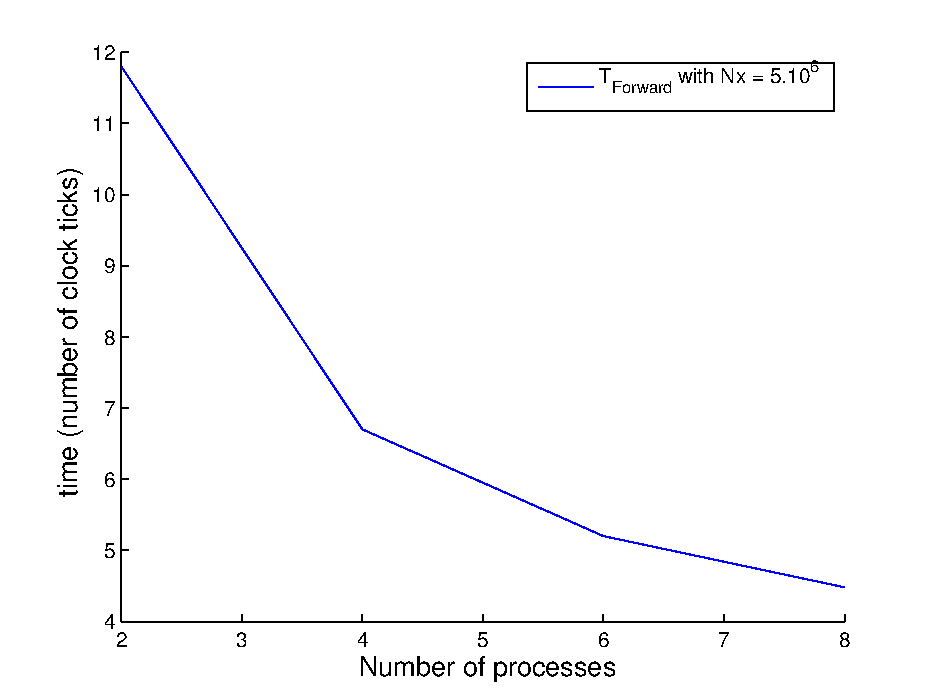
\includegraphics[width=0.8\textwidth]{figure/Forward_CB2.pdf}
\end{figure}



\hypertarget{seq-par-roukf}{}\subsection{'ReducedOrderUnscentedKalmanFilter'}\label{seq-par-roukf}


\hypertarget{seq-par-rouk-algof}{}\paragraph{Algorithm}\label{seq-par-roukf-algo}

Sampling:\\
  $ x_{h}^{(i)a} = x_h^a + L_h\sqrt{U_h^{-1}}I^{(i)} \textrm{, } \quad 1\leq i \leq p+1 $\\
  Prediction:\\
  $ x_{h+1}^f = E_\alpha(\mathcal{M}_{h}(x_{h+1}^{(*)a})) $\\
  $ x_{h+1}^{(i)f} = \mathcal{M}_{h}(x_{h}^{(i)a})$\\
  $ L_{h+1} = [x_{h+1}^{(*)f}]D_\alpha [V^*]^T \in \mathcal{M}_{n,p} $\\

  Update:\\
  $ y_{h+1}^{(i)} = \mathcal{H}_{h+1}(x_{h+1}^{(i)f})$\\
  $ \{HL\}_{h+1} = [y_{h+1}^{*}]D_\alpha [V^*]^T$\\
  $ U_{h+1} = P_{\alpha}^V +  \{HL\}_{h+1}^T R_{h+1}^{-1} \{HL\}_{h+1} \in \mathcal{M}_{p}$\\
  $ x_{h+1}^a = x_{h+1}^f + L_{h+1}U_{h+1}^{-1}\{HL\}_{h+1}^T R_{h+1}^{-1} (y_{h+1}-E_\alpha(y_{h+1}^{(*)}))$\\




\hypertarget{seq-par-roukf-ds}{}\paragraph{Distributed Structure in 'ReducedOrderUnscentedKalmanFilter'}\label{seq-par-roukf-ds}


The goal is that no variable of the model state size is allocated by any process. The concerned variables are  $x^a$, $L \in \mathcal{M}_{N_{state}, N_{sigma\_point}}$ and $ [x^{(*)f}] \in \mathcal{M}_{N_{state}, N_{reduced}}$.


\begin{itemize}

\item The state vector is a distributed dense vector whose management is delegated to the model (see Section \ref{seq-par-dm-sv}). The model state access are performed thanks to Model$::$GetState and Model$::$StateUpdated methods.

\item The sensitivity matrix $L$ is a row distributed dense matrix whose management is delegated to the model. The model is responsible for defining a a row distribution compatible with the one of the state vector (see Section \ref{seq-par-dm-cm}). The $L$ access is performed using Model$::$GetStateErrorVarianceProjector method.

\item The matrix $ [x^{(*)f}]$ must be defined as a distributed dense matrix which distribution is compatible with the one of the matrix $L$. Since the matrix  $ [x^{(*)f}]$ is peculiar to the ROUKF algorithm, its management can't be delegated to the model. Thus, it is necessary to allocate this matrix in the data assimilation method. $ [x^{(*)f}]$ construction requires two information: the type of the matrix (dense distributed) and the distribution over the processes ($[x^{(*)f}]$ distribution compatible with $L$ distribution).


$ [x^{(*)f}]$ construction must be modular: ROUKF implementation must be the same in sequential and in parallel.


\par \textcolor{red}{Specification of $ [x^{(*)f}]$ type}\\

In PETSc, the types of the structures are managed dynamically. Every matrix has the same static type 'Mat', the real type of the matrix is defined during the execution by the following function call:

\begin{frame_cpp}
Mat A;
MatSetType(A, MATMPIDENSE);
\end{frame_cpp}


Indeed, PETSc is written in C language, thus template function can't be defined for linear algebra operations. In Seldon the type of the matrices and vectors are statics. The type of $[x^{(*)f}]$ is the same as the one of $L$. It is no longer required to call any function to specify the type. (The management of the types in Verdandi is detailed in Section \ref{seq-par-type})

\par \textcolor{red}{Distribution of $ [x^{(*)f}]$}\\

The distribution of  $ [x^{(*)f}]$ is performed during the allocation. The distribution of $L$ must be provided to the constructor of matrix $[x^{(*)f}]$.



Allocation of a sequential matrix of  $\mathcal{M}_{m, n}$ :
\begin{frame_cpp}
Matrix<double> A;
A.Reallocate(m, n);
\end{frame_cpp}
Allocation of a parallel matrix of  $\mathcal{M}_{m, n}$  with a distribution of $mlocal$ rows on the local process:
\begin{frame_cpp}
Matrix<double> A;
A.Reallocate(m, n, mlocal);
\end{frame_cpp}

In order to have the same code in sequential and in parallel, the following template function is defined:
\begin{frame_cpp}
template <class Model, class T, class Prop, class Storage, class Allocator>
void Allocate(const Model& model, Matrix<T, Prop, Storage, Allocator>& A, int n, int m)
{
	A.Reallocate(m, n);
}
\end{frame_cpp}

This template function is overloaded for distributed dense matrices:
\begin{frame_cpp}
template <class Model, class T, class Prop, class Allocator>
void Allocate(const Model& model, Matrix<T, Prop, PETScMPIDense, Allocator>& A, int n, int m)
{
	A.Reallocate(m, n, model.GetLocalM());
}
\end{frame_cpp}


The allocation of  $ [x^{(*)f}]$ is perfumed in ROUKF by the following call:
\begin{frame_cpp}
Allocate(model_, X_i, Nstate, Nsigma_point);
\end{frame_cpp}

So, the implementation of ROUKF is the same in sequential and in parallel. In sequential, this implementation does not required the addition of any methods to the model interface. In parallel, the model should defined the method Model$::$GetLocalM()
which provides the number of local rows in the $L$ distribution.

\end{itemize}


\hypertarget{seq-par-roukf-p}{}\paragraph{Performance}\label{seq-par-roukf-p}

The proposed implementation enables to apply the ROUKF algorithm to a distributed model.  No variable of the model state size is allocated by any process. Thus the memory complexity is divided by the number of processes used.

Concerning the time performance, during the prediction step:

\begin{itemize}
 \item the computation  $ x_{h+1}^{(i)f} = \mathcal{M}_{h}(x_{h}^{(i)a})$ has the same speed up as the one of the model.
 \item the computation  $ L_{h+1} = [x_{h+1}^{(*)f}]D_\alpha [V^*]^T $ has a speed up equal to the number of processes.
 \end{itemize}
During the update step :
\begin{itemize}
\item the computation  $ x_{h+1}^a = x_{h+1}^f + L_{h+1}U_{h+1}^{-1}\{HL\}_{h+1}^T R_{h+1}^{-1} (y_{h+1}-E_\alpha(y_{h+1}^{(*)})) $ has a speed up equal to the number of processes.\\
\end{itemize}

The performances of the ROUKF algorithm are introduced in Figure  \ref{fig:roukf_time}.


\begin{figure}
  \caption{Simulation time of the sequential  ROUKF applied to the 'PetscClampedBar' model with $N_{state} = 5.10^6$}
  \label{fig:roukf_time}

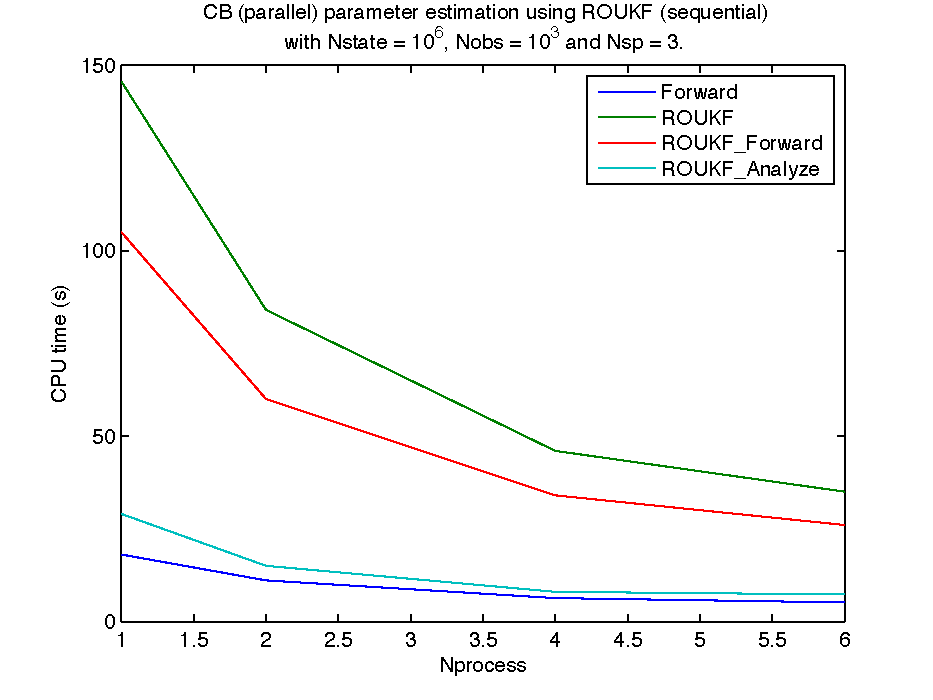
\includegraphics[width=0.8\textwidth]{figure/ROUKF_Seq_CB_Par_2.pdf}
\end{figure}



\hypertarget{seq-par-ep}{}\subsection{Example Programs}\label{seq-par-ep}

The example programs are located in the  verdandi/example/petsc\_clamped\_bar directory.


\hypertarget{seq-par-ep-c}{}\paragraph{Compilation}\label{seq-par-ep-c}


\par \textcolor{red}{Dependencies}\\


\textbf{OpenMPI}\\

\begin{itemize}

\item Download the following archive:\\
\href{http://www.open-mpi.org/software/ompi/v1.6/}{http://www.open-mpi.org/software/ompi/v1.6/}.

\item  Extract the archive and execute the following command in the source directory:

\begin{frame_bash}
$ ./configure   \
     CC=/usr/bin/gcc-4.2 \
     CPP=/usr/bin/cpp-4.2 \
     CXX=/usr/bin/g++-4.2 \
     F77=/usr/bin/gfortran \
     FC=/usr/bin/gfortran \
     F90=/usr/bin/gfortran \
     CFLAGS=-m64 \
     CXXFLAGS=-m64 \
     FFLAGS=-m64 \
     FCFLAGS=-m64 \
     LDFLAGS=-m64 \
\end{frame_bash}

\end{itemize}


\textbf{PETSc-3.3}\\

\begin{itemize}

\item Download the following archive:\\
\href{http://www.mcs.anl.gov/petsc/download/index.html}{http://www.mcs.anl.gov/petsc/download/index.html}.

\item  Extract the archive and execute the following command in the source directory:

\begin{frame_bash}
$ export PETSC_DIR=/Users/Shared/Library/Petsc
$ export PETSC_ARCH=macosx-10.7-debug
$ python config/configure.py  CXXFLAGS=-m64   CFLAGS=-m64  FCFLAGS=-m64  FFLAGS=-m64  LDFLAGS=-m64  --with-debugging=yes  --with-dynamic-loading  --with-shared-libraries  --with-parmetis-include=/Users/Shared/Library/ParMetis  --with-parmetis-lib="-L/Users/Shared/Library/ParMetis -lparmetis -lmetis" --with-metis-include=/Users/Shared/Library/Metis/64/Lib  --with-metis-lib="-L/Users/Shared/Library/Metis/64 -lmetis"  --with-superlu_dist-lib="-L/Users/Shared/Library/SuperLUDIST/lib -lsuperlu_dist"  --with-superlu_dist-include=/Users/Shared/Library/SuperLUDIST/SRC  --with-scalapack-lib="-L/Users/Shared/Library/SCALAPACK -lscalapack"  --with-scalapack-include=/Users/Shared/Library/SCALAPACK/SRC  --with-blacs-lib="-L/Users/Shared/Library/BLACS/LIB -lblacs -lblacsCinit -lblacsF77init"  --with-blacs-include=/Users/Shared/Library/BLACS/SRC  --with-mumps-include=/Users/Shared/Library/Mumps/include/ --with-mumps-lib="-L/Users/Shared/Library/Mumps/lib/ -ldmumps -lzmumps -lmumps_common -lpord -lgfortran" --with-mpi-dir=/Users/Shared/Library/OpenMPI
\end{frame_bash}

\end{itemize}


\par \textcolor{red}{Example Programs}\\


Compile the program \textbf{generate\_observation.cpp}:

\begin{frame_bash}
$ scons generate_observation mpi=yes
\end{frame_bash}

Then compile the program \textbf{reduced\_order\_unscented\_kalman\_filter.cpp}:
\begin{frame_bash}
$ scons reduced_order_unscented_kalman_filter mpi=yes
\end{frame_bash}



\hypertarget{seq-par-ep-o}{}\paragraph{Observation}\label{seq-par-ep-o}


Since no observations are given yet, we have to generate some. Execute the following command:

\begin{frame_bash}
$ mpirun -n 2 generate_observation configuration/truth.lua
\end{frame_bash}

to run the model with the initial conditions described in truth.lua, without data assimilation. This should generate a result file  \textbf{truth-state\_forecast.bin}  in the directory \textbf{example/result}. This file store the state (displacement, velocity, $\theta_f$) trajectory.
The generated state (displacement, velocity, $\theta_f$) will serve as observations for the assimilation.



\hypertarget{seq-par-ep}{}\paragraph{Data Assimilation with 'ReducedOrderUnscentedKalmanFilter'}\label{seq-par-ep}


To use the ROUKF method, execute the following command:

\begin{frame_bash}
$ mpirun -n 4 reduced_order_unscented_kalman_filter configuration/assimilation.lua
\end{frame_bash}

All processes are assigned to the model. The results should be the same as those obtained in sequential.

\hypertarget{par-par}{}\section{Parallel Method applied to Parallel Model}\label{par-par}


\hypertarget{par-par-pr}{}\subsection{Parallel 'ReducedOrderUnscentedKalmanFilter'}\label{par-par-pr}


\hypertarget{par-par-pr-mc}{}\paragraph{MPI Communicator}\label{par-par-pr-mc}


The objective is to apply the parallel ROUKF algorithm introduced in Section \ref{par-seq} on  a distributed model. We want to implement the capabilities in Verdandi to instantiate several models in parallel, and to assign several processes to each model task. A possible solution consist in using the grid topology provided by MPI:


\begin{itemize}

\item each process is defined in a MPI processor grid.

\item each process is identified by its coordinates in the grid. Figure \ref{fig:mpi_grid} represents an example of a mapping table of process rank and their corresponding grid coordinates.

\item  for each row of the grid,  a communicator containing the subgrid that includes the processes of the row is created. For instance,  in Figure \ref{fig:mpi_grid}, the group of the second row communicator is composed of processes 4, 5, 6 and 7 from $MPI\_COMM\_WORLD$ . Process 0 in second row communicator is the same as process 4 in $MPI\_COMM\_WORLD$, process 1 the same as process 5...

\item for each column of the grid,  a communicator containing the subgrid that includes the processes of the column is created.

\end{itemize}

\begin{figure}
  \caption{$4*4$ MPI Processor Grid }
  \label{fig:mpi_grid}
  \centering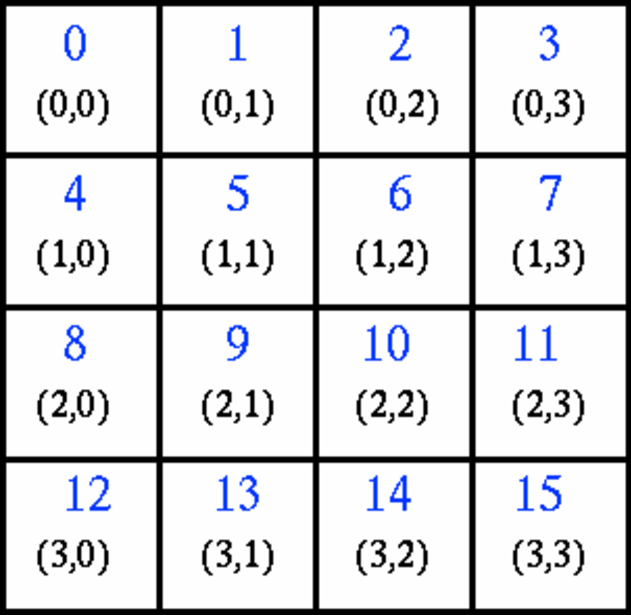
\includegraphics[width=0.4\textwidth]{figure/grid.pdf}

\end{figure}



Each column communicator correspond to an instance of model. In Figure \ref{fig:mpi_grid}, there is 4 instance of model. The first column communicator, composed of processes 0, 4, 8 and 12, is assigned to the first model instance. Then, the second column communicator is assigned to the second model instance...

Some changes  about the configuration of MPI communicators in the distributed model may be required. Indeed, the distributed model are not allowed to performed computations in the global MPI communicator $MPI\_COMM\_WORLD$. To enable several parallel model instances, $MPI\_COMM\_WORLD$ has to be replaced by a communicator of disjoint process sets in which each of the model instance operates. The column communicators to be assigned to the model instances are generated by the data assimilation method. These communicators are assigned to the model instances thanks to the following method:

\begin{frame_cpp}
namespace Verdandi
{


    //! This class is a model template.
    class ModelTemplate: public VerdandiBase
    {
        public:
            ...
            // Parallel model.
#ifdef VERDANDI_WITH_MPI
            void SetMPICommunicator(MPI_Comm& mpi_communicator);
#endif
            ...
    }

}
\end{frame_cpp}

The row communicators enable the parallel ROUKF algorithm to update its distributed variables $x^a$, $L \in \mathcal{M}_{n,p}$ and $ [x^{(*)f}] \in \mathcal{M}_{n,r}$.


\hypertarget{par-par-pr-a}{}\paragraph{Algorithm}\label{par-par-pr-a}

This Section describes the parallel ROUKF algorithm applied to a parallel model. The processes are mapped to a process grid by using row-major order (see Section \ref{par-par-pr-mc}).


\par \textbf{Initialization}

  \begin{itemize}

 \item First column  of the MPI grid (processes 0, 4, 8, 12; instance of model 0) allocates matrix $L$.\\

 \end{itemize}

 \par  \textbf{Sampling}


 \begin{itemize}

  \item First column  of the MPI grid computes  $ x_{h}^{(i)a} = x_h^a + L_h\sqrt{U_h^{-1}}I^{(i)} \textrm{, } \quad 1\leq i \leq p+1 $.

  \item First column  of the MPI grid distributes particles  $ x_{h}^{(i)a} $ over all columns.\\

 \end{itemize}

  \par  \textbf{Prediction}

   \begin{itemize}

  \item Each column  of the MPI grid computes in parallel  $ x_{h+1}^{(i)f} = \mathcal{M}_{h}(x_{h}^{(i)a})$ with its local particles.

  \item Each column of the MPI grid sends its local particles  $ x_{h+1}^{(i)f}$ to the first column.

   \item Each column of the MPI grid  computes in parallel  $ y_{h+1}^{(i)} = \mathcal{H}_{h+1}(x_{h+1}^{(i)f})$.

    \item Each column of the MPI grid sends its local particles   $ y_{h+1}^{(i)} = \mathcal{H}_{h+1}(x_{h+1}^{(i)f})$ to the first column.

  \item First column  of the MPI grid computes  $ L_{h+1} = [x_{h+1}^{(*)f}]D_\alpha [V^*]^T $.


 \end{itemize}

 \par  \textbf{Update}\\

 \begin{itemize}

 \item First column  of the MPI grid computes $ \{HL\}_{h+1} = [y_{h+1}^{*}]D_\alpha [V^*]^T$.

 \item  First column  of the MPI grid computes  $ U_{h+1} = P_{\alpha}^V +  \{HL\}_{h+1}^T R_{h+1}^{-1} \{HL\}_{h+1}$.

  \item First column  of the MPI grid computes $ x_{h+1}^a = x_{h+1}^f + L_{h+1}U_{h+1}^{-1}\{HL\}_{h+1}^T R_{h+1}^{-1} (y_{h+1}-E_\alpha(y_{h+1}^{(*)}))$.\\

 \end{itemize}



\hypertarget{par-par-ep}{}\subsection{Example Programs}\label{par-par-ep}


The example programs are located in the  verdandi/example/petsc\_clamped\_bar directory.


\hypertarget{par-par-ep-c}{}\paragraph{Compilation}\label{par-par-ep-c}


First of all, the preprocessor variable $ VERDANDI\_WITH\_MPI $ has to be defined in files  \textbf{reduced\_order\_extended\_kalman\_filter.cpp} and \textbf{reduced\_order\_unscented\_kalman\_filter.cpp}:

\begin{frame_cpp}
#define VERDANDI_DEBUG_LEVEL_4
#define SELDON_WITH_BLAS
#define SELDON_WITH_LAPACK

#define VERDANDI_WITH_ABORT
#define VERDANDI_DENSE

#define VERDANDI_WITH_MPI

#if defined(VERDANDI_WITH_MPI)
#include <mpi.h>
#endif


#include "Verdandi.hxx"
#include "seldon/SeldonSolver.hxx"

#include "model/PetscClampedBar.cxx"
#include "observation_manager/PetscLinearObservationManager.cxx"
#include "method/ReducedOrderUnscentedKalmanFilter.cxx"


int main(int argc, char** argv)
{

    VERDANDI_TRY;

    ...
}
\end{frame_cpp}

Compile the program \textbf{generate\_observation.cpp}:

\begin{frame_bash}
$ scons generate_observation mpi=yes
\end{frame_bash}

Then compile the program \textbf{reduced\_order\_unscented\_kalman\_filter.cpp}:
\begin{frame_bash}
$ scons reduced_order_unscented_kalman_filter mpi=yes
\end{frame_bash}



\hypertarget{par-par-ep-o}{}\paragraph{Observation}\label{par-par-ep-o}


Since no observations are given yet, we have to generate some. Execute the following command:

\begin{frame_bash}
$ mpirun -n 2 generate_observation configuration/truth.lua
\end{frame_bash}

to run the model with the initial conditions described in truth.lua, without data assimilation. This should generate a result file  \textbf{truth-state\_forecast.bin}  in the directory \textbf{example/result}. This file store the state (displacement, velocity, $\theta_f$) trajectory.
The generated state (displacement, velocity, $\theta_f$) will serve as observations for the assimilation.


\hypertarget{par-par-ep}{}\paragraph{Data Assimilation with 'ReducedOrderUnscentedKalmanFilter'}\label{par-par-ep}


The parameters of the ROUKF method are described in the configuration file  \textbf{configuration/assimilation.lua}.

It is necessary to define the dimension of the MPI grid. The number of model instances and the number of processes assigned to each model instance must be defined:

\textbf{assimilation.lua}\\
\begin{frame_lua}
-- Simulation with assimilation using ROUKF.
reduced_order_unscented_kalman_filter = {

 	...

   mpi_grid = {

      -- The number of processes for each model task.
      Nrow = 2,
      -- The number of model tasks.
      Ncol = 3
   }

}

\end{frame_lua}

To use the ROUKF method, execute the following command:

\begin{frame_bash}
$ mpirun -n 6 reduced_order_unscented_kalman_filter configuration/assimilation.lua
\end{frame_bash}

\textbf{Warning:} The number of processes must be equal to $mpi\_grid.Nrow * mpi\_grid.Nco$.


The results should be the same as those obtained in sequential.

\hypertarget{par-par-p}{}\section{Performance}\label{par-par-p}


\begin{figure}
  \caption{PetscClampedBar parameter estimation using ROUKF (parallel) with $N_{state} = 10^5$ and $N_{observation} = 10^4$ }

  \vspace{1cm}

  \label{fig:roukf_par_time}
  \centering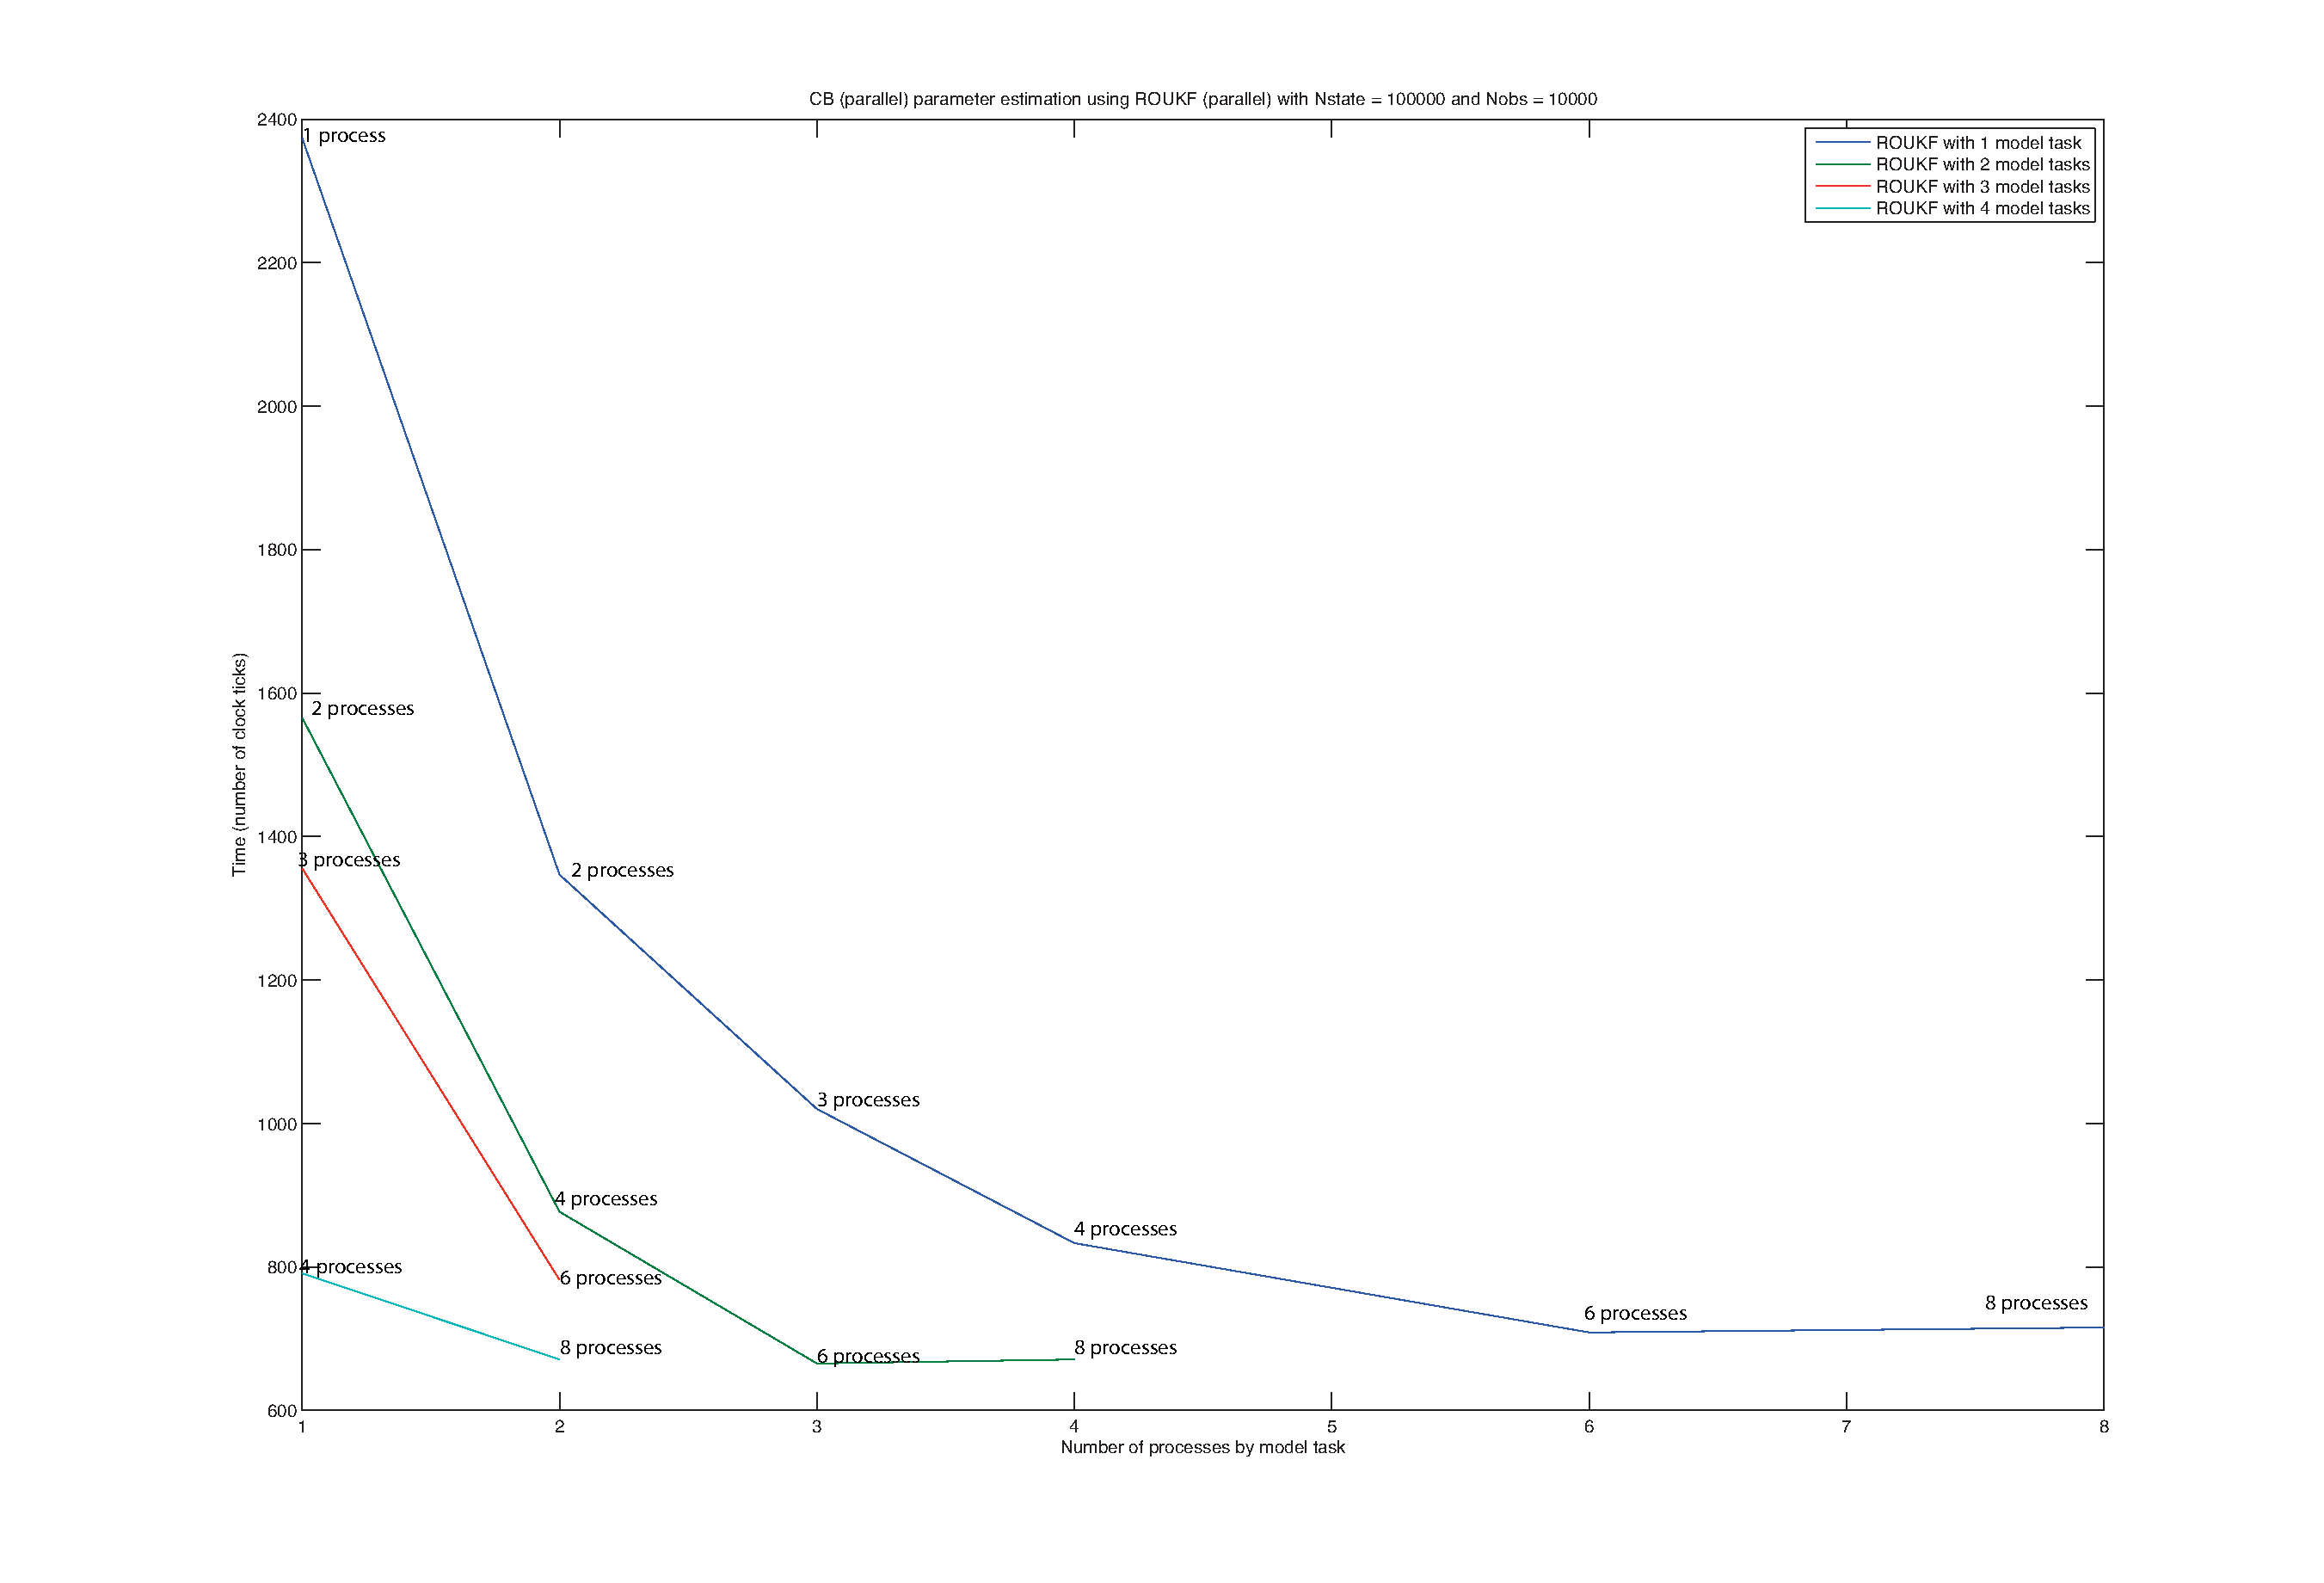
\includegraphics[width=1.\textwidth]{figure/roukf_par_3_test.pdf}
\end{figure}


We can see in Figure \ref{fig:roukf_par_time} that when the number of processes is less than or equal to four, it is more in efficient to instantiate only one model and to assign all processes to this instance. On the other hand, when the number of processes increases, the most effective is to own
several model instances:

\begin{itemize}

\item when the number of processes is equal to sox, the most efficient is to define two model instances running on three processes.

\item when the number of processes is equal to sox, the optimal configuration is to have two model instances running on four processes.

\end{itemize}


As intended, this second level of parallelism provides a better scalability. At the fist level of parallelism, when the efficiency of ROUKF algorithm decreases, this second level of parallelism contributes to better take advantage of the  available computation resources.
